
\documentclass[conference]{IEEEtran}
\usepackage[utf8]{inputenc}
\usepackage[english]{babel}
\usepackage{graphicx}
\usepackage{amsmath}
\usepackage{hyperref}
\usepackage[numbers]{natbib}
\usepackage{geometry}
\usepackage{multirow}
\usepackage{float}
\usepackage{tabularx}
\usepackage{booktabs}
\geometry{margin=1in}

\title{Comparing machine learning and deep learning models to moderate inappropriate messages on social media.}
\author{Nicolas Bedoya Figueroa \\
Daniel Escalante Pérez \\
Marilyn Stephany Joven Fonseca \\
Eder Leandro Carbonero Baqueron \\}
\date{\today}
\pagestyle{plain} 

\begin{document}

\maketitle
\begin{abstract}
Aquí va el resumen del artículo, una breve descripción del problema, la metodología y los resultados.
\end{abstract}

\section{Introduction}
A detailed and clear contextualization of the problem is presented below, specifying the area in which it is framed—namely, digital communication and social media—and highlighting its relevance. The main objective is to analyze and mitigate the presence of hate speech on social media platforms through machine learning techniques.

Over the past couple of decades, with the advancement of technology and the internet, social media platforms have become increasingly relevant. These platforms have enabled the easier dissemination of information, its democratization, and global connectivity.

In 2024, this growth continued. Facebook led in the number of monthly active users, reaching over 3 billion—something no other platform has achieved to date. YouTube followed with 2.5 billion users, while Instagram and WhatsApp occupied third place, each with around 2 billion users. As a result, social media platforms also generate substantial revenue; for example, Facebook alone generates more than 80 billion USD annually. These figures clearly show the significance of social media platforms, both in terms of user base and economic impact.

However, social media has also introduced new challenges. With the ability to post content at any time and on nearly any topic, hate speech directed at individuals or groups has become increasingly prevalent. This type of speech has begun to impact society. In January 2023, attacks were carried out on Brazilian government buildings, and on January 6, 2021, the United States Capitol was stormed. Both incidents occurred after certain groups spread dangerous rhetoric and false claims against others.

A deeper analysis of this issue on platforms such as Facebook and Instagram reveals the following figures:

\begin{figure}[htbp]
    \centering
    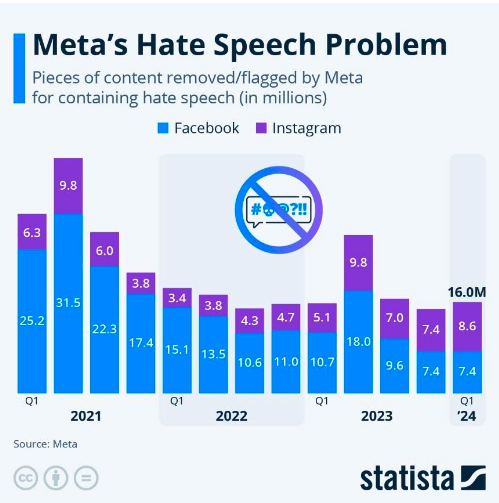
\includegraphics[width=0.9\linewidth]{images/MetaHateSpeechProblem.png}
    \caption{Meta's hate speech problem. Source: \cite{zandt2024}.}
    \label{fig:meta_hate_speech_problem}
\end{figure}
 
As observed, millions of pieces of content are removed every year due to the presence of hate speech in various forms.

Additionally, on the platform X (formerly Twitter), there has been a notable increase in such comments. Hate speech has generally risen by 50\%, while transphobic, homophobic, and racist comments have increased by 260\%, 30\%, and 42\%, respectively.

This highlights the significant relevance of hate speech in the social context, particularly on social media. Effectively identifying and removing such comments is a fundamental task that social platforms must undertake.

Therefore, the goal of this project is to develop \textit{Machine Learning} and \textit{Deep Learning} models to effectively classify comments in English, since this is one of the most commonly used languages. For instance, 55\% of tweets on X are published in English.

The aim is to compare the implemented models and determine which one delivers the best results.


\section{Related Work}

The problem of detecting toxicity and hate speech has been addressed by a variety of authors, each proposing interesting solutions. These authors have applied different methodologies, preprocessing techniques, models, and embeddings that have yielded varying results, but overall, they highlight the potential of using Machine Learning and Deep Learning to solve the problem.

In \cite{fieri2023offensive}, Fieri and Suhartono aimed to perform automatic moderation using Machine Learning and Deep Learning to combat the rapid spread of offensive language on the internet. Building on previous research, they explored the best combination of models to construct an ensemble model that used soft voting. This form of voting determines the probability of each class for each estimator in order to make the overall prediction.

Regarding the methodology, a dataset from Twitter was used, and cleaning was performed to remove URLs, user mentions, and punctuation. Subsequently, Easy Data Augmentation was applied to balance the datasets using techniques such as synonym replacement, random insertion, random swap, and random deletion. The dataset was tokenized. Then, for Deep Learning, embedding using GloVe was applied, and for Machine Learning, TF-IDF and sentiment analysis with Valence Aware Dictionary and Sentiment Reasoner (VADER) were used.

For Machine Learning, the models used were: Random Forest, Naive Bayes, Decision Tree, Logistic Regression, AdaBoost, and KNN. These models were trained using cross-validation, and based on the F1-score, the top 3 and top 5 were selected to build models with soft voting. For Deep Learning, CNN, LSTM, Bi-LSTM, GRU, and Bi-GRU were used. These networks were trained and grouped, taking one version each of LSTM and GRU along with CNN \cite{fieri2023offensive}.

Regarding the results, it was found that Random Forest was the best Machine Learning model, achieving an F1-score of 92.685%, and the best ensemble consisted of Random Forest, Decision Tree, Logistic Regression, AdaBoost, and Naive Bayes, reaching 92.750\%. In Deep Learning, Bi-LSTM achieved the best results with an F1-score of 93.560\%, and the best ensemble reached 93.818\%. The study concludes by noting that there may still be interesting combinations yet to be explored \cite{fieri2023offensive}.

% Luego en el cuerpo:
\begin{table}[!t]
\caption{Performance comparison of Machine Learning and Deep Learning models (F1-score)}
\label{tab:results}
\centering
\begin{tabularx}{\linewidth}{|l|X|c|}
\hline
\textbf{Category} & \textbf{Model(s)} & \textbf{F1-score (\%)} \\ \hline
\multirow{2}{*}{Machine Learning} 
  & Best single model: Random Forest & 92.685 \\ \cline{2-3}
  & Best ensemble: RF, DT, LR, AdaBoost, NB & 92.750 \\ \hline
\multirow{2}{*}{Deep Learning} 
  & Best single model: Bi-LSTM & 93.560 \\ \cline{2-3}
  & Best ensemble: CNN, Bi-LSTM, GRU & 93.818 \\ \hline
\end{tabularx}
\end{table}

\vspace{0.5em}

As shown in Table~\ref{tab:results}, the Deep Learning models, particularly Bi-LSTM and its ensembles, outperform the Machine Learning counterparts by a small margin. This suggests that recurrent architectures and their combinations are effective for detecting toxic comments. However, the high performance of ensemble methods in both categories indicates that combining models can enhance predictive accuracy.

In \cite{bonetti2023comparison}, Bonetti et al., with an objective similar to that in \cite{fieri2023offensive}, seek to compare three methods frequently used in NLP challenges: Logistic Regression, Random Forest, and Support Vector Machine, along with topic modeling techniques (Latent Semantic Analysis - LSA and Latent Dirichlet Allocation - LDA), as well as the Transformer architecture, for the task of toxicity detection.

In this research, TF-IDF and word embeddings were used. Two datasets were created: one with basic cleaning and lemmatization, and another similar one but without stop words and with emojis translated into words.

For traditional Machine Learning models, TF-IDF was used with Logistic Regression and Random Forest. After experimenting with these models in their basic state, LDA with three topics was applied on the data to detect relevant aspects and improve the training of the two mentioned algorithms. Subsequently, LSA was used to reduce the dataset dimensionality and extract the main topics, combining it with SVM using a radial kernel \cite{bonetti2023comparison}.

Finally, the Transformer architecture with BERTweet was employed to compare Machine Learning with Deep Learning. For BERTweet, fine-tuning was performed on its final layer. A variant with a binary classification neural network on top was also tested, training the entire model, and another version training only the binary classification layers.

In the logistic regression experiment, an F1-score of 0.9073 was achieved using the first dataset. With Random Forest, a score of 0.9011 was obtained using the second dataset with the following hyperparameters: 100 estimators, a maximum depth of 80, and 10 samples required to split a node. SVM + LSA achieved 0.9112 using 5000 dimensions in LSA and C = 4.

Using BERTweet, 0.9140 was reached with 4 epochs, a learning rate of 2 $\times$ 10$^{-5}$ with the Adam optimizer, and a hidden dropout probability of 0.3 in the model with fine-tuning on the head layer \cite{bonetti2023comparison}.

Regarding LDA, the best model was logistic regression with the first dataset, achieving an F1-score of 0.9046. The research concludes that the task is difficult due to a highly changing environment. Nevertheless, it can be said that among the investigated models, high results were achieved, with logistic regression offering the best balance between performance and computational cost \cite{bonetti2023comparison}.

Following similar objectives, Toktarova et al. in \cite{toktarova2023hate} sought to contribute to the development of tools and strategies to combat hate speech on social networks, aiming to create a healthy environment. To this end, they investigated and compared multiple methods from both Deep Learning and Machine Learning in the context of hate speech on Twitter.

In this research, after performing cleaning preprocessing on three datasets, TF-IDF and Word2Vec were used to embed the texts. For Machine Learning exploration, decision trees, Naive Bayes, KNN, and SVM were used. For Deep Learning, LSTM, Bi-LSTM, and CNN were employed.

From the results, it was shown that the most valuable methods were Deep Learning ones, highlighting Bi-LSTM, which achieved an F1-score of 0.899 on one of the datasets used.

The research concludes that traditional Machine Learning fails to capture context, unlike some Deep Learning architectures. However, the latter are more prone to overfitting, require large volumes of data, are harder to train, and computationally expensive.

One final consideration, which is very interesting, concerns the importance of achieving metrics that minimize both false positives and false negatives, to avoid the unjustified suppression of freedom of expression \cite{toktarova2023hate}.


\section{Theorical framework}
This study presents a comprehensive methodological framework for the detection of hate speech on Twitter, integrating both machine learning and deep learning approaches. The process began with an extensive data preprocessing pipeline to ensure data consistency, clean noisy text, and address class imbalance using Easy Data Augmentation (EDA)~\cite{wei2019eda}. This included standard text normalization techniques—such as stopword removal and stemming—as well as more advanced steps like automated spelling correction and synonym expansion.

Subsequently, multiple classification models were implemented and evaluated. For traditional machine learning, models such as Support Vector Machines (SVM), Logistic Regression, and Multinomial Naive Bayes were applied, providing baseline performances and interpretability advantages. On the deep learning side, we implemented architectures including Convolutional Neural Networks (CNN) and Gated Recurrent Units (GRU), both trained on pretrained embeddings to capture contextual linguistic features.

In addition, transformer-based language models were explored, notably RoBERTa, for which both zero-shot evaluation and supervised fine-tuning were performed. The fine-tuning involved training a classification head on top of RoBERTa’s pretrained layers using our balanced dataset.

This comparative methodology allows for a fair assessment across heterogeneous architectures, evaluating their strengths and limitations under a consistent experimental setup inspired by previous works~\cite{fieri2023offensive,almeida2023comparison}.

\subsection{Machine learning Methods}
This section describes the classification methods used in this study. Each represents a different approach within supervised learning.

\subsubsection{Logistic Regression}
\textbf{Definition}
Logistic regression is a statistical model used to predict the probability of a binary class. It is efficient for linear problems and serves as a baseline for comparison with more complex models.

To reference one of the earliest formulations of the model, we draw upon the perspective presented in \textit{The Regression Analysis of Binary Sequences} by D. R. Cox (1958), which introduced a rigorous statistical framework for the analysis of binary outcomes. In this work, both dependent and independent variables are explicitly identified, and the probability of a binary event is modeled using a logistic transformation of the predictors. Dependent variables are represented as binary categorical variables, typically coded as 0 and 1, which enables the analysis of how one or more explanatory variables influence the likelihood of an event of interest. Through illustrative examples, the author demonstrates how the model can be estimated using maximum likelihood methods, thereby establishing a methodological foundation that continues to be widely applied in fields such as biostatistics, the social sciences, and machine learning \citep{cox1958logistic}.

Given the capabilities offered by the model, it has been selected for use in this study. However, prior to its implementation, we will review some previous approaches used in earlier research.

As one of the initial and relevant approaches, the study presented in the article "Offensive Language Detection Using Soft Voting Ensemble Model" \citep{supert2023offensive} incorporates logistic regression as part of its ensemble strategy. The article emphasizes the use of L2 regularization, which enhances the precision of offensive language classification by mitigating overfitting. Furthermore, the model's simplicity is highlighted as a significant advantage, enabling efficient implementation even with limited computational resources—demonstrating its usefulness and versatility within the set of evaluated classifiers.

The research article titled "Comparison between Machine Learning and Deep Learning Approaches for the Detection of Toxic Comments on Social Networks" \citep{bonetti2023comparison} employs logistic regression once again, combining it with two semantic modeling techniques: Latent Semantic Analysis (LSA) and Latent Dirichlet Allocation (LDA). These methods will be further discussed in the following paragraphs. Notably, the study reports a prediction accuracy exceeding 91\%, highlighting the competitiveness of traditional approaches compared to more complex deep learning models.

\subsubsection{Na\"ive Bayes}

\noindent
Naïve Bayes is a simple and quick probabilistic classifier that uses Bayes' theorem, assuming independence between features. It works well in text classification, especially for high-dimensional data and sparse input, which is common in natural language processing (NLP). Naïve Bayes calculates the probability of a class based on specific terms, effectively detecting hate speech by analyzing occurrences of certain words.

Recent studies, including Hate Speech Detection in Social Networks using Machine Learning and Deep Learning Methods \citep{hate2022bonetti} highlight Naïve Bayes' effectiveness on platforms like Twitter, achieving a precision of 0. 832 and a recall of 0. 863, resulting in an F1-score of 0. 851. Another study by Asif et al. (2024), while noting Naïve Bayes' limitations in capturing context, recognizes its computational efficiency and acceptable recall, making it a practical choice compared to deep learning models.
\subsubsection{SVM (Support Vector Machines)}

SVM (Support Vector Machines) is a machine learning method mainly used for classification tasks. Its main goal is to find the best hyperplane that separates the classes and maximizes the margin with the closest points from each class. This process involves identifying the support vectors, which are the closest points to the classification hyperplane. A common technique used with SVM is the use of kernels. With kernels, data points are transformed into a new space that might be linearly separable, improving classification results. There is a variety of kernels with different transformation approaches to choose from. An important hyperparameter for this algorithm is “C,” which refers to a regularization term that controls the trade-off between margin maximization and misclassifications~\cite{geeksforgeeks_svm}.

\subsubsection{XGBoost}

One of the models that drew the most attention when choosing which to use for the toxicity classification task was XGBoostClassifier. According to \cite{xgboost2016}, XGBoost stands for Extreme Gradient Boosting and is based on the use of multiple decision and regression trees to create an ensemble method with greater predictive power. In this model, scores are assigned to examples according to the leaf in which they are classified by each tree, and then those scores are summed. This approach is similar to that used in Random Forests, with the difference that training is performed through Boosting. The goal of the method is to learn both the structure and the scores of the trees. In each training iteration, it seeks to find the tree that contributes the most to optimizing the objective, which can vary depending on the task. It can be said that the trees in the ensemble method complement each other to solve the task for which the training is performed.

In \cite{fieri2023offensive}, the ensemble methods tested were AdaBoost and Random Forest, achieving an accuracy of 95.518 using Random Forest. On the other hand, in \cite{bonetti2023comparison}, using this same classifier, an accuracy of 91.88 was reached. Finally, in \cite{toktarova2023hate}, also with this classifier, an accuracy of 85.1 was obtained. Based on these results, these scores can be taken as a reference and the search for some improvement can be established.


\subsection{Deep Learning Methods}
Deep learning is a subset of machine learning that uses artificial neural networks with many layers to automatically learn complex patterns from large amounts of data.

\subsubsection{MLP}
An MLP (Multi-Layer Perceptron) is the simplest and most fundamental form of neural networks and deep learning. It builds on the concept of neurons, grouping them into layers and then stacking those layers. Each neuron performs a simple weighted sum, but when organized in layers, the input data can be transformed into a new feature space. MLP architectures typically consist of an input layer, multiple hidden layers, and an output layer, which is responsible for producing the final result. These networks are usually fully connected, meaning that every output from one layer is passed to each node in the next layer. Layers are paired with activation functions that introduce non-linearity and help transform outputs into a desired range, such as between 0 and 1 to represent a probability. MLPs are trained using an ``error'' metric, such as cross-entropy loss, and optimized using algorithms like gradient descent through backpropagation across all weights~\cite{mlp_gfg}.

\subsubsection{Convolutional Neural Networks (CNNs)}
In the reviewed studies~\cite{bonetti2023comparison,fieri2023offensive}, Convolutional Neural Networks (CNNs) have been employed as an efficient deep learning approach for the detection of offensive language and toxic comments. Their ability to extract spatial patterns from text embeddings enables the identification of relevant structures within input sequences, leading to effective classification. However, although CNNs exhibit competitive performance, the studies also emphasize that their effectiveness may be surpassed by models capable of capturing full-sequence context, such as bidirectional recurrent neural networks or transformer-based models, particularly when dealing with complex or ambiguous natural language inputs.

\subsubsection{BI-LSTM}

\noindent
\cite{toktarova2023hate} BI-LSTM (Bidirectional Long Short-Term Memory) is a type of sequential neural network that allows working with data composed of different elements ordered in a sequence, such as text. This type of network can make predictions about parts of the sequence based on what has been seen so far or on the entire input. It is an improvement over LSTM networks, which, like recurrent networks, use output values from previous steps in the sequence. However, it differs by dividing the network's responsibilities into different flow control gates. Additionally, it is capable of maintaining both long-term memory and a hidden state, which allows it to respond appropriately to the current step in the sequence. BI-LSTMs process the input both forward and backward, thus capturing future and past context at each step. In \cite{fieri2021soft}, using BI-LSTM, an accuracy of 90.2 was achieved; meanwhile, in \cite{bonetti2023comparison}, 96.102 was reached.


\subsubsection{GRU}

\noindent
Gated recurrent Units (GRUs) are part of the recurrent neural network (RNNs) designed to work with sequential data. GRUs use a gating mechanisms with update and reset gates to control flow information over time, which allows the model to remember or forget information effectively. This helps to capture relationships in text while having a less complex structure like for example LSTM networks.

GRUs have shown strong performance when in use for hate speech detection in social media. In a Comparison between Machine Learning and Deep Learning Approaches for the Detection of Toxic Comments on Social Networks \citep{bonetti2023comparison}, GRUs are compared with LSTM and CNN models, in this case GRUs performed well in accuracy and adaptability, especially with diverse and informal language. Another study Hate Speech Detection in Social Networks using Machine Learning and Deep Learning Methods \citep{faisal2023hate} highlighted GRUs efficiency in recognizing patterns in toxic comments, achieving a high F1-score of 0.907 compared to traditional methods. GRUs are efficient for real-time content moderation, balancing performance and speed.

\subsubsection{roBERTa}
RoBERTa is a bidirectional pretrained encoder based on BERT, but trained on a larger amount of data and with longer sequences. BERT itself is based on the encoder component of the Transformer architecture, which generates vector representations by considering both the past and future context of the sequence elements. The pretrained knowledge of the model can be reused for other tasks by simply adding a classification head and fine-tuning the pretrained weights to solve the new problem. In \cite{bonetti2023comparison}, BERTweet was used — a model similar to RoBERTa but specifically trained on Twitter data — achieving an accuracy of 92.38.

\section{Methodologies and experiments}
\label{sec:methodologies}
\subsection{Machine learning Methods}
This section describes the classification methods used in this study. Each represents a different approach within supervised learning.

\subsubsection{Pre processing and Data Augmentation}
\label{sec:preprocessing}
To implement the methods based on Machine learning or deep learning for hate speech detection on Twitter, a thorough data preprocessing procedure was carried out to balance the classes in the dataset. First, the two target categories were identified: \textit{hate speech} and \textit{no hate speech}, encoded as 1 and 0, respectively. Various text cleaning techniques were then applied, including the removal of special characters, URLs, mentions, Twitter-specific symbols, spelling correction, stopword removal, stemming, as well as the elimination of duplicate records and null values. Additionally, the vocabulary was enriched through synonym validation and expansion. To address the inherent class imbalance, the Easy Data Augmentation (EDA) technique was applied, which allowed for the generation of a balanced dataset, ultimately saved in a CSV file named \texttt{balanced\_data.csv}~\cite{wei2019eda}.

The preprocessing approach adopted in this study shares several similarities with previous works such as those by Fieri et al.~\cite{fieri2023offensive} and Almeida et al.~\cite{almeida2023comparison}, particularly in terms of text data cleaning and preparation for hate speech detection tasks. As in these studies, common techniques were applied, including the removal of textual noise (mentions, URLs, symbols), lexical normalization, and dimensionality reduction through the use of stopwords and stemming. However, our approach integrates additional steps that are not consistently addressed in those works, such as automated spelling correction, semantic validation using synonyms, and the application of data augmentation techniques like Easy Data Augmentation (EDA). This last aspect represents a significant difference, as the reviewed studies often rely on direct undersampling or oversampling, whereas our methodology emphasizes the synthetic generation of new samples. This can contribute to greater dataset diversity and model robustness during training, regardless of the architecture employed~\cite{wei2019eda}.


\subsection{Logistic Regression}
\subsubsection{Definition}
Logistic regression is a statistical model used to predict the probability of a binary class. It is efficient for linear problems and serves as a baseline for comparison with more complex models.

To reference one of the earliest formulations of the model, we draw upon the perspective presented in \textit{The Regression Analysis of Binary Sequences} by D. R. Cox (1958), which introduced a rigorous statistical framework for the analysis of binary outcomes. In this work, both dependent and independent variables are explicitly identified, and the probability of a binary event is modeled using a logistic transformation of the predictors. Dependent variables are represented as binary categorical variables, typically coded as 0 and 1, which enables the analysis of how one or more explanatory variables influence the likelihood of an event of interest. Through illustrative examples, the author demonstrates how the model can be estimated using maximum likelihood methods, thereby establishing a methodological foundation that continues to be widely applied in fields such as biostatistics, the social sciences, and machine learning \citep{cox1958logistic}.

Given the capabilities offered by the model, it has been selected for use in this study. However, prior to its implementation, we will review some previous approaches used in earlier research.

As one of the initial and relevant approaches, the study presented in the article "Offensive Language Detection Using Soft Voting Ensemble Model" \citep{supert2023offensive} incorporates logistic regression as part of its ensemble strategy. The article emphasizes the use of L2 regularization, which enhances the precision of offensive language classification by mitigating overfitting. Furthermore, the model's simplicity is highlighted as a significant advantage, enabling efficient implementation even with limited computational resources—demonstrating its usefulness and versatility within the set of evaluated classifiers.

The research article titled "Comparison between Machine Learning and Deep Learning Approaches for the Detection of Toxic Comments on Social Networks" \citep{bonetti2023comparison} employs logistic regression once again, combining it with two semantic modeling techniques: Latent Semantic Analysis (LSA) and Latent Dirichlet Allocation (LDA). These methods will be further discussed in the following paragraphs. Notably, the study reports a prediction accuracy exceeding 91%, highlighting the competitiveness of traditional approaches compared to more complex deep learning models.



\subsection{Deep Learning Methods}
Deep learning is a subset of machine learning that uses artificial neural networks with many layers to automatically learn complex patterns from large amounts of data.

\subsubsection{roBERTa}
RoBERTa is a bidirectional pretrained encoder based on BERT, but trained on a larger amount of data and with longer sequences. BERT itself is based on the encoder component of the Transformer architecture, which generates vector representations by considering both the past and future context of the sequence elements. The pretrained knowledge of the model can be reused for other tasks by simply adding a classification head and fine-tuning the pretrained weights to solve the new problem. In \cite{bonetti2021hate}, BERTweet was used — a model similar to RoBERTa but specifically trained on Twitter data — achieving an accuracy of 92.38.

\subsubsection{Methodology XGBoost}

The methodology used for the XGBoostClassifier began by loading the [CLS] token embeddings generated by RoBERTa, that is, the vector that summarizes the entire text sequence. After this, the data was split into 80\% for training and 20\% for testing. This split resulted in 38,152 examples available for training. Subsequently, a parameter grid was defined to conduct hyperparameter tuning. The search focused on the number of estimators, maximum tree depth, and minimum child weight. To find the best values, a grid search with 3-fold cross-validation was used.

In addition to this search, other hyperparameters were set manually. For example, 80\% of the data was used in each boosting round, and in each tree and node, a sample of features was selected such that its size was proportional to the square root of the total number of features, as recommended in \cite{Chen2016XGBoost}.

For training, 50\% of the dataset was used to perform the hyperparameter search, as doing it on the entire training set would have been computationally too expensive. Once the best hyperparameters were found, the model was trained on the full training set and then evaluated.

To evaluate the model, a classification report was generated that measured precision, recall, F1-score, and accuracy. Additionally, a confusion matrix was presented to more clearly observe the trend of the data toward true positives or misclassification.

\subsubsection{Methodology BI-LSTM}

For the model based on the BI-LSTM architecture, the full embeddings generated by the roBERTa model were used, and the architecture shown in Figure~\ref{fig:bilstm_architecture}, as recommended in \cite{zhang2018deep}, was implemented. This architecture was trained using the Adam optimizer for 200 epochs, storing the checkpoint that achieved the highest accuracy on the validation set. This validation set accounted for 15\% of the data, as did the test set, while the remaining 70\% was used for training. 

After training, the best checkpoint was restored and performance evaluation was carried out. The model was assessed using the same metrics as with the XGBoostClassifier: precision, recall, F1-score, accuracy, and the confusion matrix.

\begin{figure}[htbp]
  \centering
  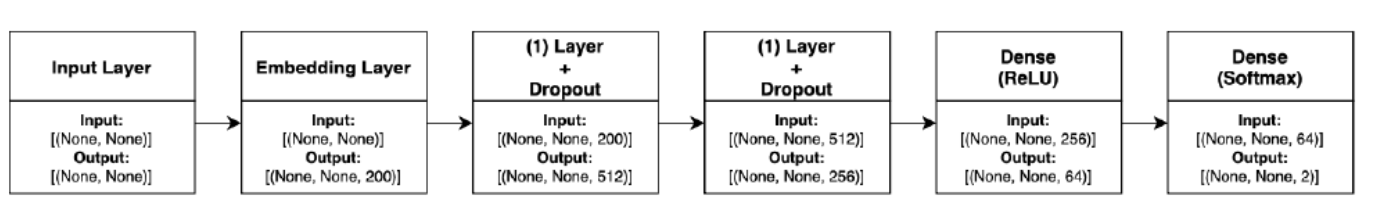
\includegraphics[width=0.45\textwidth]{images/bilstm_architecture.png}
  \caption{BI-LSTM architecture used in the model.}
  \label{fig:bilstm_architecture}
\end{figure}

\subsubsection*{Fine-tuning methodology for RoBERTa}

To fine-tune the pretrained \texttt{twitter-roBERTa} model and adapt it to solve the classification task, we used the tokenized input data, which had not yet been embedded by the model. These data were split into 70\%, 15\%, and 15\% for the training, validation, and test sets, respectively, similar to the BI-LSTM architecture. 

Next, we created a three-layer classification head following the architecture shown in Figure~\ref{fig:roberta_finetune_architecture} \cite{liu2019roberta}. Dropout layers were added to prevent overfitting. This classification head was then integrated with the RoBERTa encoder, using the representation of the \texttt{[CLS]} token, which, as mentioned before, summarizes the input sequence.

With the full model ready, we froze the RoBERTa weights to train only the classification head. The training lasted 150 epochs, used batches of 32 samples, and employed the Adam optimizer, storing the checkpoints of the best-performing models. After this first stage, we evaluated the results and performed a second training stage, where all pretrained weights were unfrozen. This second stage was trained using a learning rate of 0.000001, the Adam optimizer, for 100 epochs, again with a batch size of 32.

To assess the best model from each training stage as well as the untrained model, we used precision, recall, F1-score, accuracy, and the confusion matrix.

\begin{figure}[htbp]
  \centering
  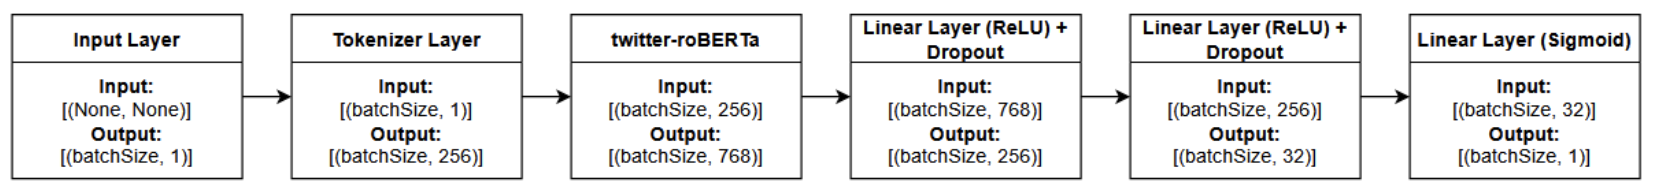
\includegraphics[width=0.45\textwidth]{images/roberta_finetune_architecture.png}
  \caption{Architecture used for fine-tuning twitter-RoBERTa.}
  \label{fig:roberta_finetune_architecture}
\end{figure}


\subsubsection{BI-LSTM}

\noindent
\cite{toktarova2023hate} BI-LSTM (Bidirectional Long Short-Term Memory) is a type of sequential neural network that allows working with data composed of different elements ordered in a sequence, such as text. This type of network can make predictions about parts of the sequence based on what has been seen so far or on the entire input. It is an improvement over LSTM networks, which, like recurrent networks, use output values from previous steps in the sequence. However, it differs by dividing the network's responsibilities into different flow control gates. Additionally, it is capable of maintaining both long-term memory and a hidden state, which allows it to respond appropriately to the current step in the sequence. BI-LSTMs process the input both forward and backward, thus capturing future and past context at each step. In \cite{fieri2021soft}, using BI-LSTM, an accuracy of 90.2 was achieved; meanwhile, in \cite{bonetti2023comparison}, 96.102 was reached.




\subsubsection{CNN Methodology}
\label{sec:cnn}

Using the Convolutional Neural Network (CNN) architecture, various configurations were explored to obtain an effective training setup. With a balanced dataset of 47,706 labeled messages now available, the data was split into two subsets: 80\% for training and 20\% for testing. The final model was structured with three hidden convolutional layers. Although deeper architectures were initially tested, they were deemed suboptimal given the relatively limited size of the dataset.

Each of the convolutional layers was followed by a ReLU (Rectified Linear Unit) activation function. ReLU is commonly used in deep learning because it introduces non-linearity by outputting zero for all negative values and keeping positive values unchanged, which helps avoid vanishing gradient problems and accelerates convergence.

To reduce the spatial dimensions and computational complexity of the model, a \texttt{MaxPooling1D} layer with a pool size of 2 was applied after each convolution. Max pooling extracts the most prominent feature within each segment of the input, effectively downsampling the representation and providing translation invariance, which is particularly useful in textual pattern recognition.

In order to prevent overfitting—an issue often encountered when training deep networks on relatively small datasets—Dropout layers with a dropout rate of 0.3 were included. Dropout randomly deactivates a fraction of neurons during training, which helps the model generalize better by discouraging co-adaptations of feature detectors.

Finally, the architecture concluded with a dense output layer using the sigmoid activation function. This function maps the output to a probability between 0 and 1, suitable for binary classification tasks like distinguishing between hate and non-hate speech.

The model was compiled and trained using the Adam optimizer, which combines the advantages of both AdaGrad and RMSProp by adapting the learning rate for each parameter. A learning rate of 0.0005 was selected to balance the speed of convergence with training stability, allowing the model to make gradual improvements without overshooting minima.

The implemented CNN model consists of three convolutional blocks followed by max pooling and dropout layers. This structure enables the progressive extraction of textual features while controlling overfitting. The Conv1D layers increase in complexity (from 64 to 256 filters), while MaxPooling1D reduces the dimensionality of the text, making processing more efficient.

The use of Dropout layers between convolutional blocks, with a dropout rate of 0.3, effectively mitigates overfitting—an important consideration given the dataset size of 47,706 samples. Subsequently, a Flatten layer transforms the three-dimensional output into a vector, which is then processed by a dense layer of 128 neurons. This dense layer accounts for the majority of the model’s parameters. Finally, a Dense output layer with a sigmoid activation function performs the binary classification.

Compared to previous studies such as those by Fieri et al. and Almeida et al., this CNN model opts for a lighter architecture focused on efficiency and local pattern extraction, avoiding more complex hybrid or recurrent architectures that are typically more computationally expensive.

During the CNN training phase, an early stopping strategy was implemented to prevent overfitting and optimize generalization. Training was initially scheduled for 30 epochs with a batch size of 32. Validation metrics were monitored continuously, resulting in automatic termination of training after 16 epochs when no sustained improvement was observed on the validation set.

At the end of training, the model achieved the following results on the training data:

\begin{itemize}
    \item Accuracy: 0.8836
    \item Loss: 0.2719
    \item Precision: 0.9430
    \item Recall: 0.8191
\end{itemize}

Regarding the validation set, the recorded metrics were:

\begin{itemize}
    \item Validation Accuracy: 0.8600
    \item Validation Loss: 0.3175
    \item Validation Precision: 0.9325
    \item Validation Recall: 0.7835
\end{itemize}

Finally, when evaluating the model on the actual test data, the following performance was obtained:

\begin{itemize}
    \item Accuracy: 0.8610
    \item Precision: 0.9190
    \item Recall: 0.7991
    \item F1 Score: 0.8549
\end{itemize}

These results demonstrate consistency across training, validation, and testing phases, indicating that the model maintains a good balance between precision and recall. Furthermore, when compared to similar models in previous studies, such as Fieri et al. (2023), the CNN architecture exhibits competitive performance with a lower structural complexity.


\subsubsection{XGBoost}

One of the models that drew the most attention when choosing which to use for the toxicity classification task was XGBoostClassifier. According to \cite{xgboost2016}, XGBoost stands for Extreme Gradient Boosting and is based on the use of multiple decision and regression trees to create an ensemble method with greater predictive power. In this model, scores are assigned to examples according to the leaf in which they are classified by each tree, and then those scores are summed. This approach is similar to that used in Random Forests, with the difference that training is performed through Boosting. The goal of the method is to learn both the structure and the scores of the trees. In each training iteration, it seeks to find the tree that contributes the most to optimizing the objective, which can vary depending on the task. It can be said that the trees in the ensemble method complement each other to solve the task for which the training is performed.

In \cite{comparison2023toxic}, the ensemble methods tested were AdaBoost and Random Forest, achieving an accuracy of 95.518 using Random Forest. On the other hand, in \cite{fieri2021soft}, using this same classifier, an accuracy of 91.88 was reached. Finally, in \cite{bonetti2021hate}, also with this classifier, an accuracy of 85.1 was obtained. Based on these results, these scores can be taken as a reference and the search for some improvement can be established.




\section{Results}
\subsection{Random Forest Results}
\label{sec:random_forest_results}

As part of the machine learning baseline models evaluated in this study, a Random Forest classifier was implemented and trained on the preprocessed dataset. This ensemble method, which operates by constructing multiple decision trees and aggregating their outputs, is known for its robustness and resistance to overfitting, especially in high-dimensional textual data. The model yielded promising results on the test set, achieving an \textbf{accuracy} of 0.8627, a \textbf{precision} of 0.8980, a \textbf{recall} of 0.8246, and an \textbf{F1-score} of 0.8597. These metrics indicate a balanced performance in detecting both hate and non-hate speech categories, demonstrating the classifier's effectiveness even in comparison with more complex deep learning approaches. In terms of interpretability and computational efficiency, Random Forest remains a strong candidate for practical deployment in moderation systems.


\subsubsection{XGBoost Results}

Following the methodology described earlier—specifically, performing grid search with cross-validation to tune hyperparameters—we found that the best values were: 500 trees, a maximum depth of 20, and a minimum child weight of 2. With these settings, an accuracy of 0.852 was achieved using only 50\% of the dataset for training. When the model was later trained using the entire training set, the accuracy increased to 0.86.

Table~\ref{tab:xgboost_classification_report} shows the classification report. It is worth highlighting that the model tends to predict the “Non-toxicity” class more frequently, as it has a higher recall compared to the positive (toxic) class, although its precision is lower. This indicates the presence of more false negatives, which also affects the recall of the positive class: more false negatives mean fewer true positives. To address this issue, a larger number of toxic examples could be included in the training data. Although this would create an imbalance, it would allow the model to better understand the class it is intended to detect and potentially improve its performance.

\begin{table}[htbp]
\centering
\caption{Classification report for XGBoost model on the test set.}
\label{tab:xgboost_classification_report}
\begin{tabular}{lcccc}
\toprule
\textbf{Class} & \textbf{Precision} & \textbf{Recall} & \textbf{F1-score} & \textbf{Support} \\
\midrule
0 (Non-toxic)   & 0.83 & 0.89 & 0.86 & 4626 \\
1 (Toxic)       & 0.89 & 0.83 & 0.86 & 4912 \\
\midrule
\textbf{Accuracy}       & \multicolumn{4}{c}{0.86} & 9538 \\
\textbf{Macro avg}      & 0.86 & 0.86 & 0.86 & 9538 \\
\textbf{Weighted avg}   & 0.86 & 0.86 & 0.86 & 9538 \\
\bottomrule
\end{tabular}
\end{table}

In Figure~\ref{fig:confusion_matrix_xgboost}, the model's confusion matrix can be observed. It reflects the quality of the model, showing a high concentration of true positives and true negatives. However, the accuracy is 86\%, and more than 1300 misclassified examples are observed in the test set. This implies that, in a production environment, there could be cases of toxicity that persist or non-toxicity cases that are unjustly censored.

\begin{figure}[H]
    \centering
    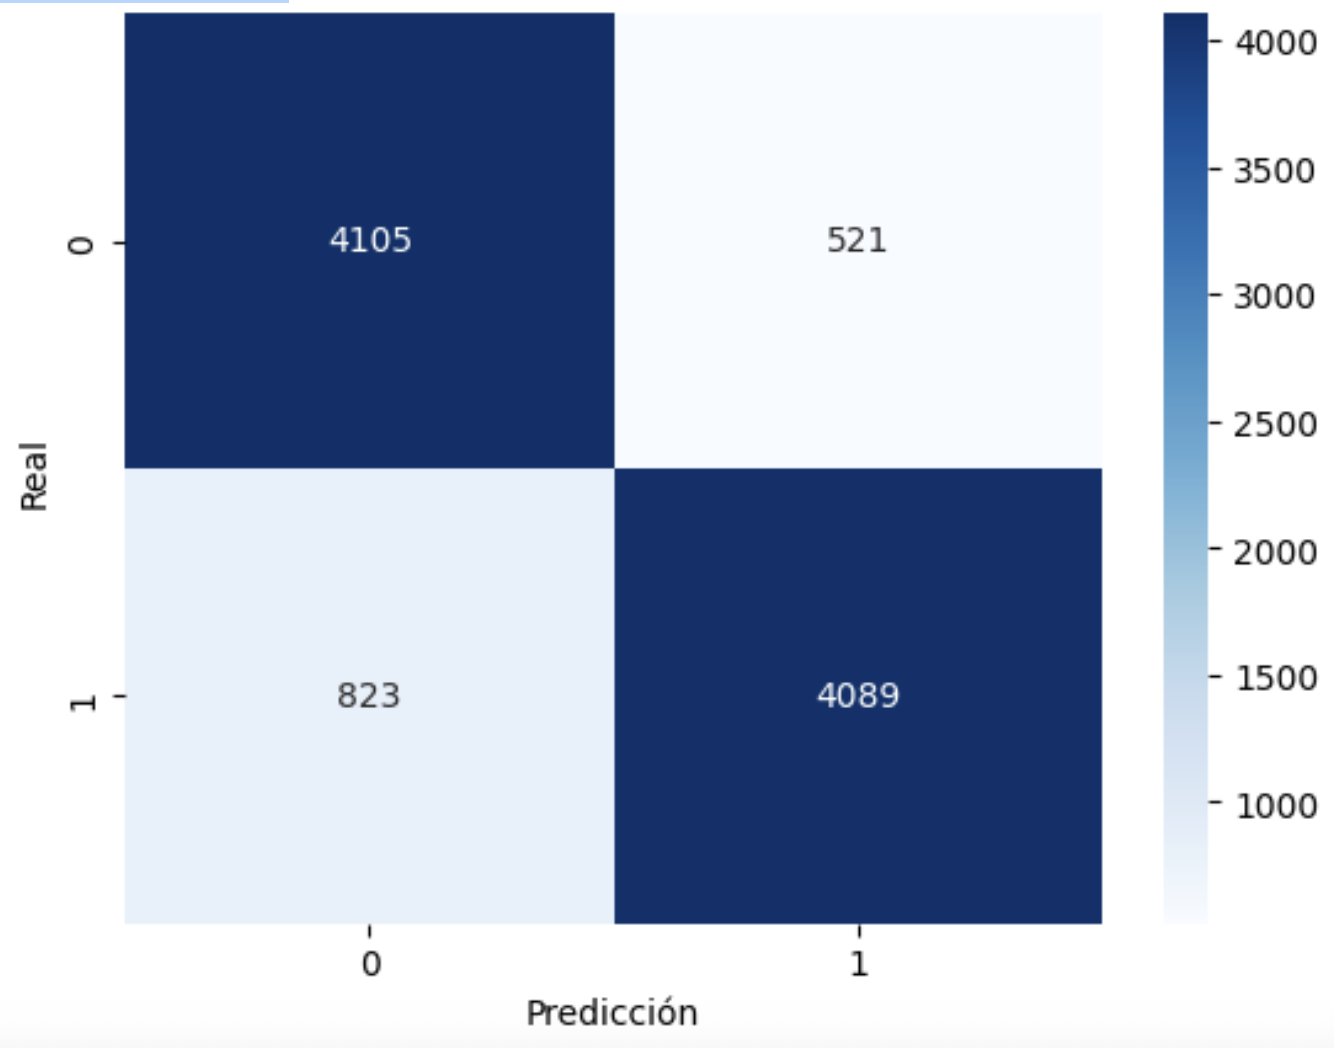
\includegraphics[width=0.45\textwidth]{images/confusion_matrix_xgboots.png} 
    \caption{Confusion Matrix for XGBoost model}
    \label{fig:confusion_matrix_xgboost}
\end{figure}

The accuracy obtained of 86\% exceeds that observed in \cite{toktarova2023hate}, although it does not exceed what was seen in \cite{bonetti2023comparison} and \cite{fieri2023offensive}.

\subsubsection{BI-LSTM Results}

After implementing the architecture recommended in \cite{fieri2023offensive} and training it for 200 epochs using Twitter-RoBERTa embeddings, the following results were obtained:

\begin{figure}[H]
    \centering
    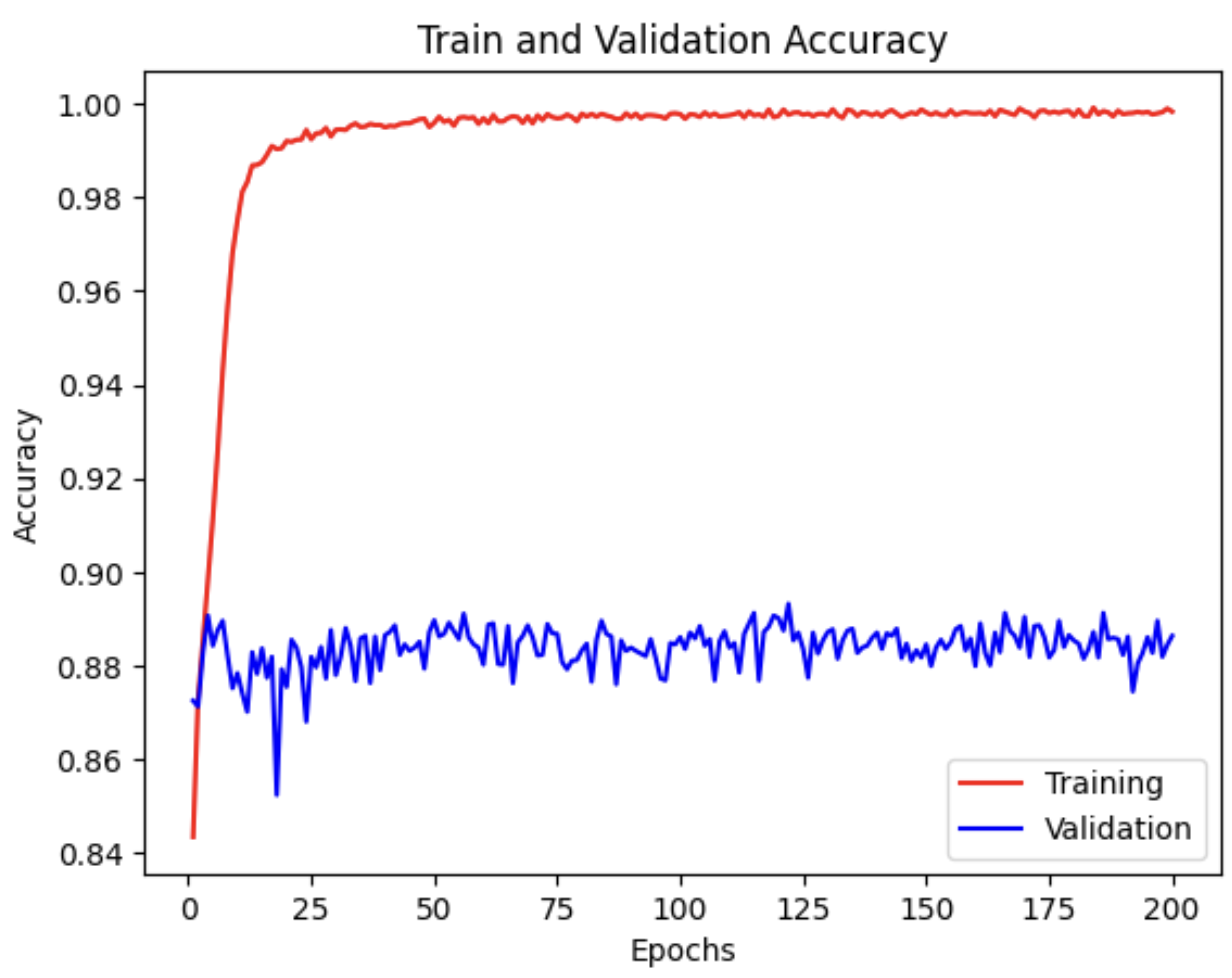
\includegraphics[width=0.45\textwidth]{images/trainingValidationAccurayBI_LSTM.png}
    \caption{Training and Validation Accuracy for BI-LSTM model using Twitter-RoBERTa embeddings}
    \label{fig:accuracy_bilstm}
\end{figure}

\begin{figure}[H]
    \centering
    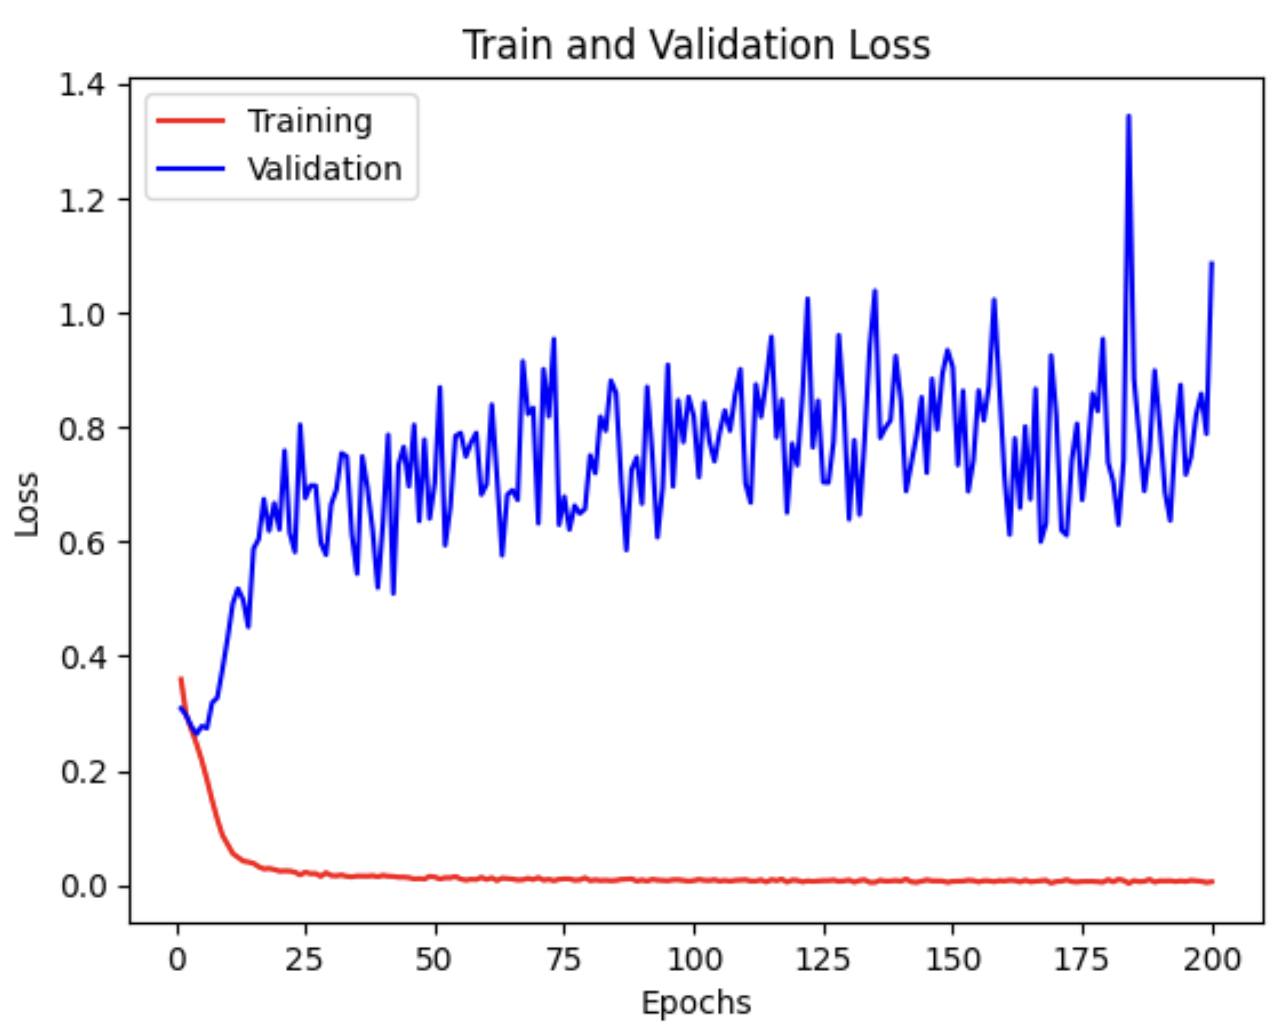
\includegraphics[width=0.45\textwidth]{images/trainingValidationLossBI_LSTM.png}
    \caption{Training and Validation Loss for BI-LSTM model using Twitter-RoBERTa embeddings}
    \label{fig:loss_bilstm}
\end{figure}

As shown in Figures \ref{fig:accuracy_bilstm} and \ref{fig:loss_bilstm}, the BI-LSTM model quickly overfits the training data. The training performance is very high, with a loss approaching 0 and an accuracy near 1. In contrast, the validation set shows worse results, with loss values ranging between 0.5 and 1.4, and accuracy stabilizing around 0.88.

Due to this oscillating behavior, with several performance spikes, a checkpoint was saved using the best validation accuracy. This peak occurred at epoch 122, achieving an accuracy of 0.89321. This represents a significant improvement compared to other results, such as those obtained with XGBoost. However, the score approaches—but does not surpass—the results reported in \cite{fieri2023offensive} and \cite{toktarova2023hate}.

\begin{table}[H]
\centering
\caption{Classification Report}
\label{tab:classification_report}
\begin{tabular}{lcccc}
\toprule
Class        & Precision & Recall & F1-score & Support \\
\midrule
0            & 0.86      & 0.93   & 0.89     & 3517    \\
1            & 0.92      & 0.86   & 0.89     & 3638    \\
\midrule
Accuracy     &           &        & 0.89     & 7155    \\
Macro Avg    & 0.89      & 0.89   & 0.89     & 7155    \\
Weighted Avg & 0.89      & 0.89   & 0.89     & 7155    \\
\bottomrule
\end{tabular}
\end{table}

In Table~\ref{tab:classification_report}, the generated classification report is shown, reflecting the same problem observed with XGBoost: many examples are predicted as "non-toxic." This is particularly evident in the reduced precision for the negative class and the lowered recall for the positive class. Nevertheless, there is a clear improvement across all metrics, approaching 90\%.

\begin{figure}[H]
    \centering
    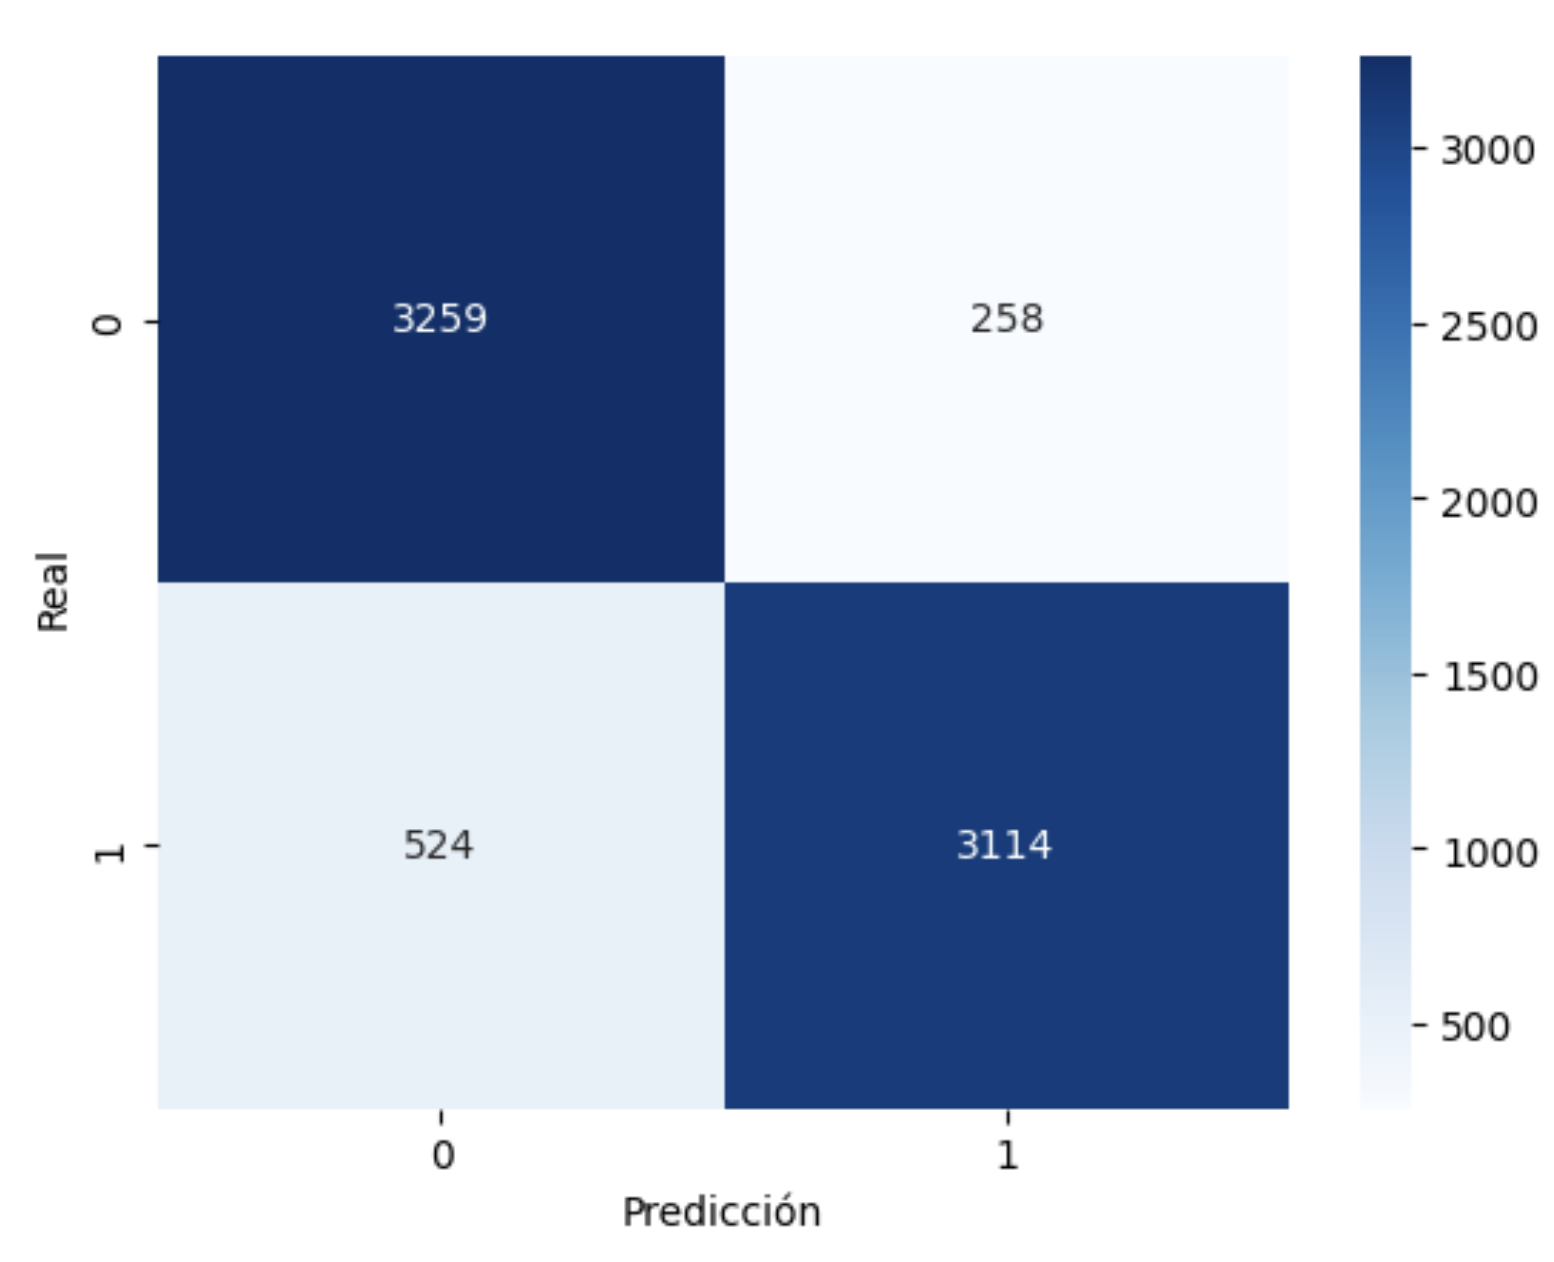
\includegraphics[width=0.45\textwidth]{images/confusion_matrix_bilstm.png}
    \caption{Confusion matrix of the BI-LSTM model}
    \label{fig:confusion_matrix_bilstm}
\end{figure}

In Figure \ref{fig:confusion_matrix_bilstm}, the confusion matrix is shown, where predictions are more focused on true positives and true negatives, with a higher proportion compared to other tested models.

\subsubsection{CNN Results}
\label{sec:cnn_results}

The CNN machine learning model was trained, as mentioned in the methodology, which allowed us to obtain a total of 3,203,969 parameters for training. After 16 epochs, the values shown in Table~\ref{tab:train_metrics} were obtained for the training and validation phases. Training stopped at epoch 16 due to early stopping. However, the final results evaluated on the test data are presented in Table~\ref{tab:test_metrics}.

We can observe that, compared to previous studies on which our work is based, the accuracy was lower; nonetheless, the obtained results indicate that overfitting was avoided during training and a proper balance between training and validation phases was achieved.

\begin{table}[h]
    \centering
    \caption{Metrics during training and validation (final epoch)}
    \label{tab:train_metrics}
    \begin{tabular}{lcc}
        \toprule
        Metric         & Training & Validation \\
        \midrule
        Accuracy       & 0.8850   & 0.8624     \\
        Loss           & 0.2608   & 0.3153     \\
        Precision      & 0.9340   & 0.9150     \\
        Recall         & 0.8344   & 0.8065     \\
        \bottomrule
    \end{tabular}
\end{table}

\begin{table}[h]
    \centering
    \caption{Final metrics on test data}
    \label{tab:test_metrics}
    \begin{tabular}{lc}
        \toprule
        Metric    & Value   \\
        \midrule
        Accuracy  & 0.8618  \\
        Precision & 0.9266  \\
        Recall    & 0.7929  \\
        F1 Score  & 0.8546  \\
        \bottomrule
    \end{tabular}
\end{table}

ssss

As shown in Figure~\ref{fig:cnn_accuracy}, the training accuracy was initially lower than the validation accuracy during the early epochs. However, the difference was not substantial—approximately four percentage points. Around epoch 16, this trend reversed, with training accuracy surpassing validation accuracy. Despite this shift, an early stopping mechanism was applied to prevent overfitting by halting the training process once the validation performance ceased to improve significantly.

\begin{figure}[H]
    \centering
    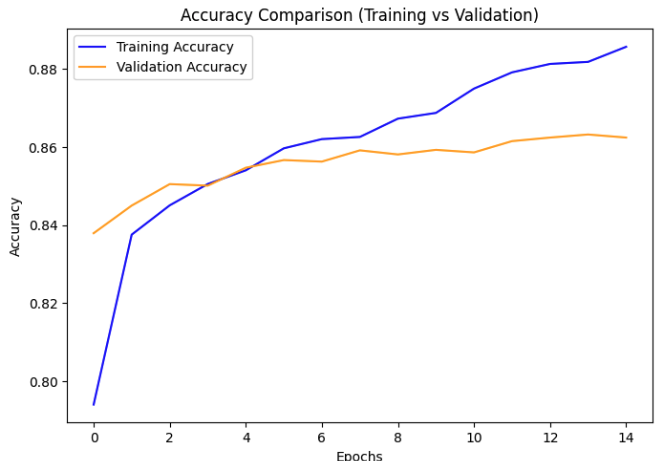
\includegraphics[width=0.45\textwidth]{images/AccuracyComparisonCNN.png}
    \caption{Accuracy comparison between training and validation for CNN model}
    \label{fig:cnn_accuracy}
\end{figure}

A similar but inverse trend can be observed in the loss curves, as shown in Figure~\ref{fig:cnn_loss}. At the beginning of training, the training loss is higher than the validation loss, with a nominal difference of approximately 0.1. As training progresses, this behavior reverses, and the training loss becomes lower than the validation loss. This indicates that while the model initially struggles more with the training data, it gradually learns to generalize, although the growing gap at later epochs may hint at overfitting, which was mitigated by applying early stopping.

\begin{figure}[H]
    \centering
    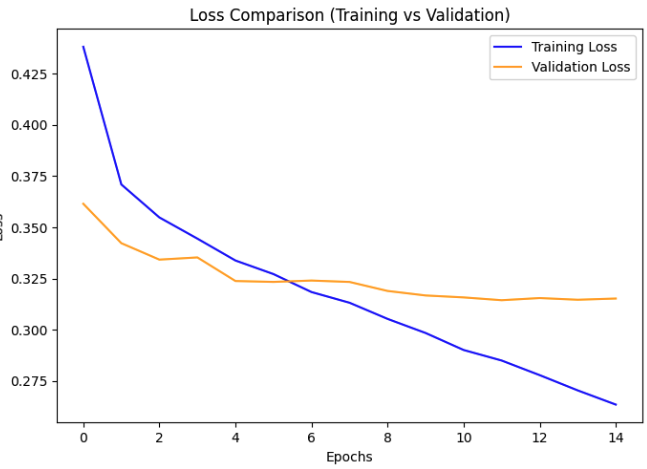
\includegraphics[width=0.45\textwidth]{images/LossComparisonCNN.png}
    \caption{Loss comparison between training and validation for CNN model}
    \label{fig:cnn_loss}
\end{figure}

In the case of precision, as shown in Figure~\ref{fig:cnn_precision}, we observe a gradual increase beginning around the second epoch. However, the precision values for the validation set fluctuate between 89\% and 94\%. This variability may be primarily attributed to the limited amount of training data available. Nevertheless, the achieved precision values can be considered favorable and promising for potential deployment in a production setting.

\begin{figure}[H]
    \centering
    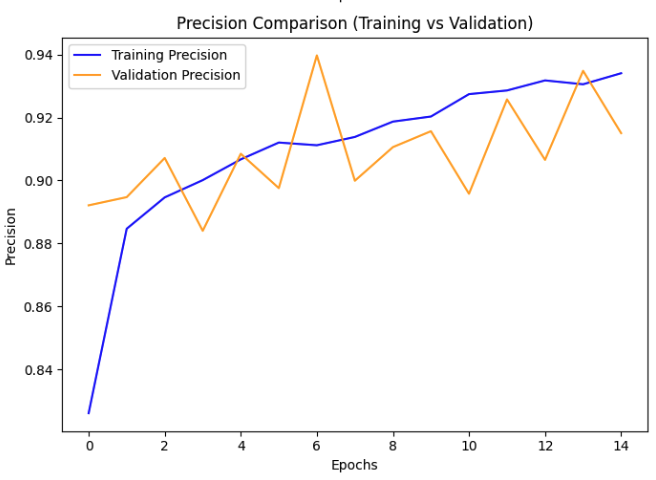
\includegraphics[width=0.45\textwidth]{images/PrecisionComparisonCNN.png}
    \caption{Precision comparison between training and validation for CNN model}
    \label{fig:cnn_precision}
\end{figure}

The recall metric, illustrated in Figure~\ref{fig:cnn_recall}, exhibits a consistent and positive upward trend during training. However, the validation recall demonstrates a more oscillatory behavior, fluctuating throughout the epochs. This variation in the validation set may indicate sensitivity to the limited dataset or variability in the model's ability to generalize recall performance.

\begin{figure}[H]
    \centering
    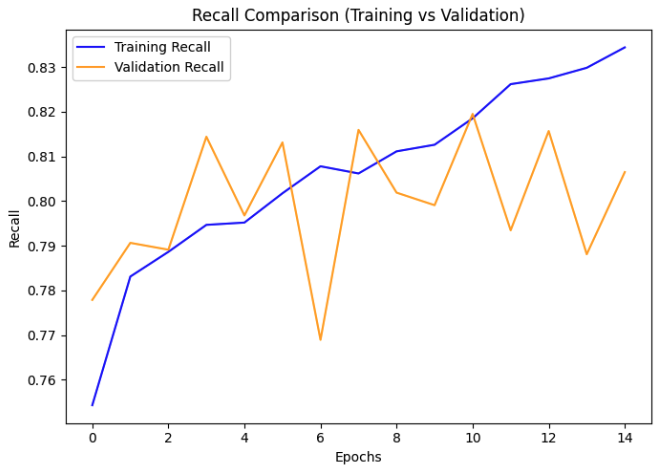
\includegraphics[width=0.45\textwidth]{images/RecallComparisonCNN.png}
    \caption{Recall comparison between training and validation for CNN model}
    \label{fig:cnn_recall}
\end{figure}
 
The confusion matrix shows that the model correctly classifies 4,347 cases as "No hate speech" and 3,875 cases as "Hate speech." However, it also presents 307 false positives (cases wrongly labeled as hate speech when they are not) and 1,012 false negatives (hate speech cases not detected). This imbalance indicates that, although the model is quite accurate, there is still significant room for improvement in detecting hate speech and reducing false negatives, which can have a considerable impact on automatic moderation.

\begin{figure}[H]
    \centering
    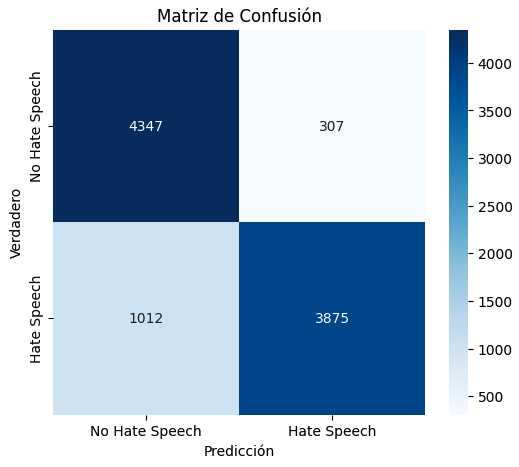
\includegraphics[width=0.45\textwidth]{images/matrixOfConfusion.png}
    \caption{Confusion matrix of the model's predictions on the test set.}
    \label{fig:confusion_matrix}
\end{figure}


\subsubsection{RoBERTa-Twitter Results}

The first step in fine-tuning RoBERTa-Twitter was to evaluate its performance without training the classification head and using the default weights, aiming to establish a baseline. Doing so yielded the classification report shown in Table~\ref{tab:classification_report_1} and the confusion matrix presented in Figure \ref{fig:confusion_matrix_roberta_shapeY_no_head}.

\begin{table}[H]
\centering
\caption{Classification Report without Training the Classification Head}
\label{tab:classification_report_1}
\begin{tabular}{lcccc}
\toprule
Class        & Precision & Recall & F1-score & Support \\
\midrule
0.0          & 0.00      & 0.00   & 0.00     & 3456    \\
1.0          & 0.52      & 1.00   & 0.68     & 3699    \\
\midrule
Accuracy     &           &        & 0.52     & 7155    \\
Macro Avg    & 0.26      & 0.50   & 0.34     & 7155    \\
Weighted Avg & 0.27      & 0.52   & 0.35     & 7155    \\
\bottomrule
\end{tabular}
\end{table}

\begin{figure}[H]
    \centering
    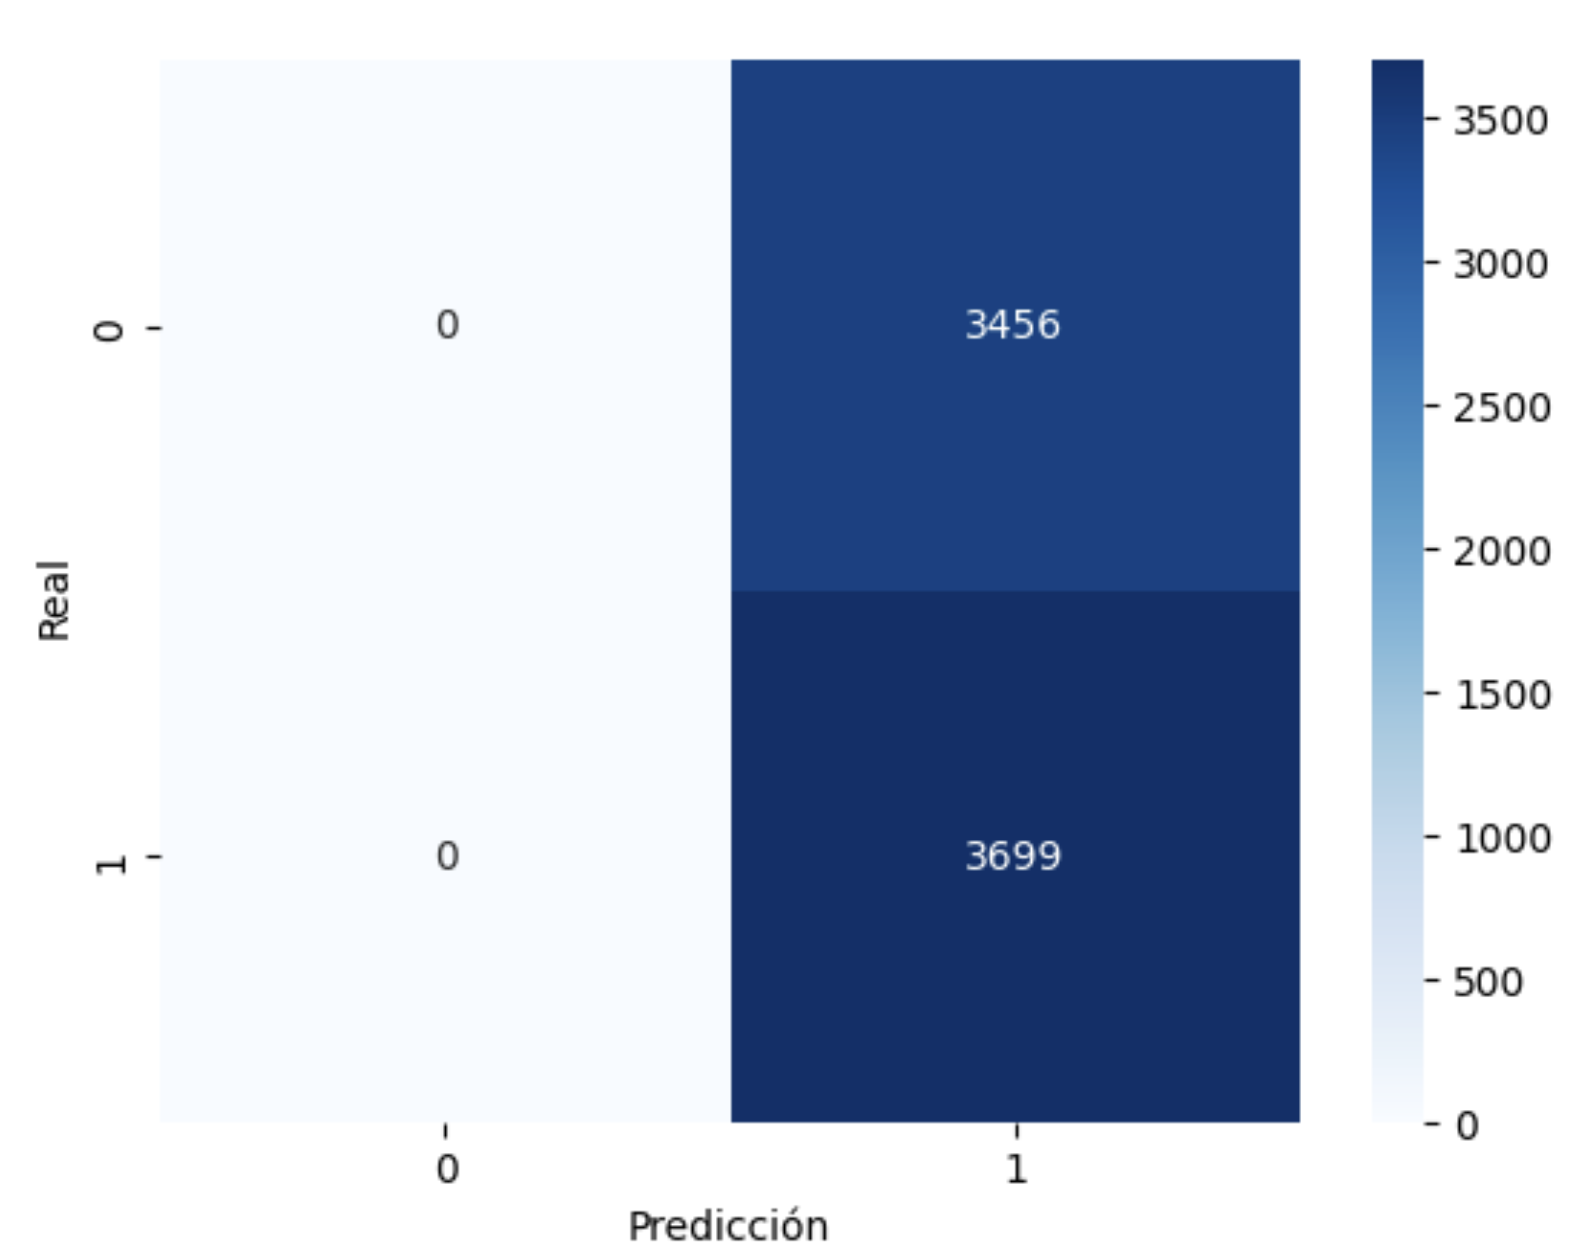
\includegraphics[width=0.45\textwidth]{images/confusion_matrix_bilstm_shapeY.png}
    \caption{RoBERTa-Twitter model confusion matrix without training the classification head}
    \label{fig:confusion_matrix_roberta_shapeY_no_head}
\end{figure}


As observed, the model predicts everything as toxic. This is because the classification head still retains its random weights and the RoBERTa-Twitter model has not yet been fine-tuned for this specific task.

Following the methodology, in the first training phase only the classification head is trained for 150 epochs. The results of this phase can be seen in Figures \ref{fig:roberta_validation_loss_finetune} and \ref{fig:roberta_accuracy_finetune}.


\begin{figure}[H]
    \centering
    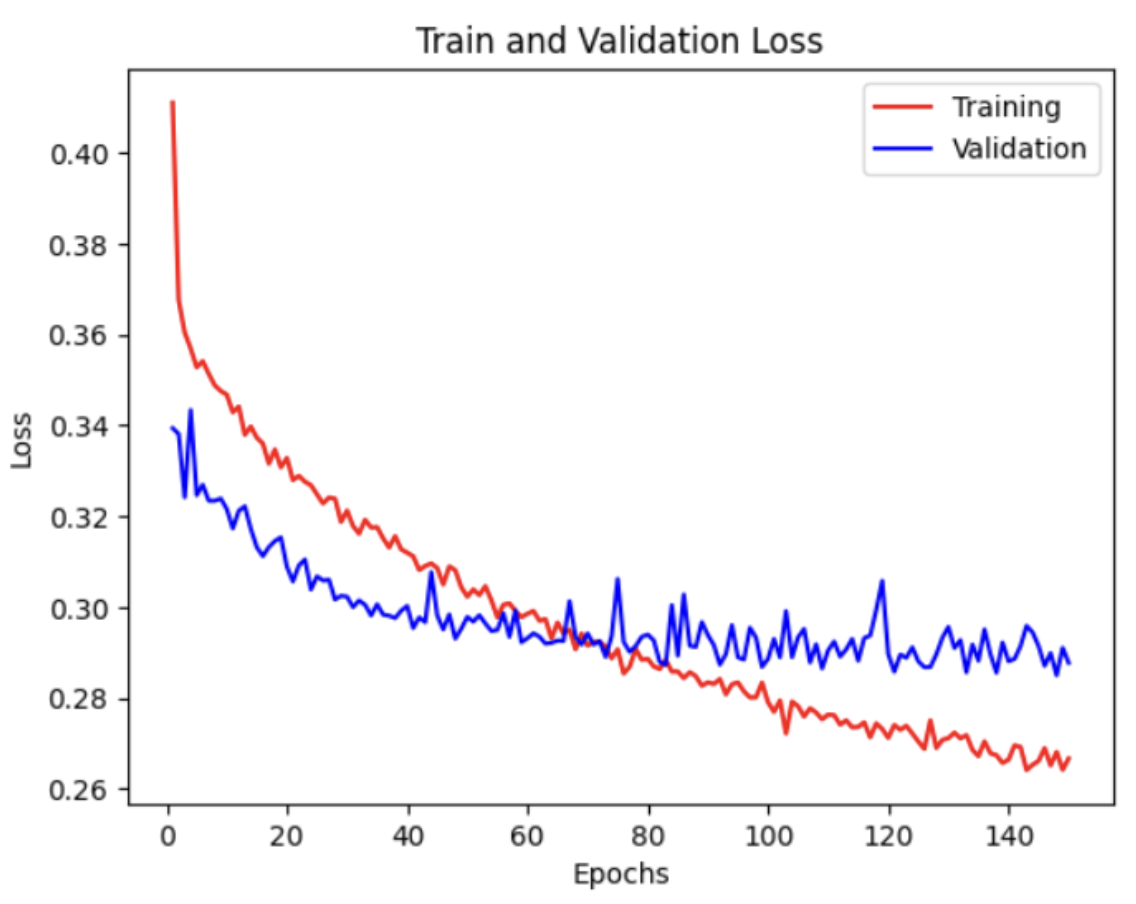
\includegraphics[width=0.45\textwidth]{images/robertaValidationLossFigureX15Epoch.png}
    \caption{Validation loss of the RoBERTa-Twitter model during classification head training (150 epochs)}
    \label{fig:roberta_validation_loss_finetune}
\end{figure}

\begin{figure}[H]
    \centering
    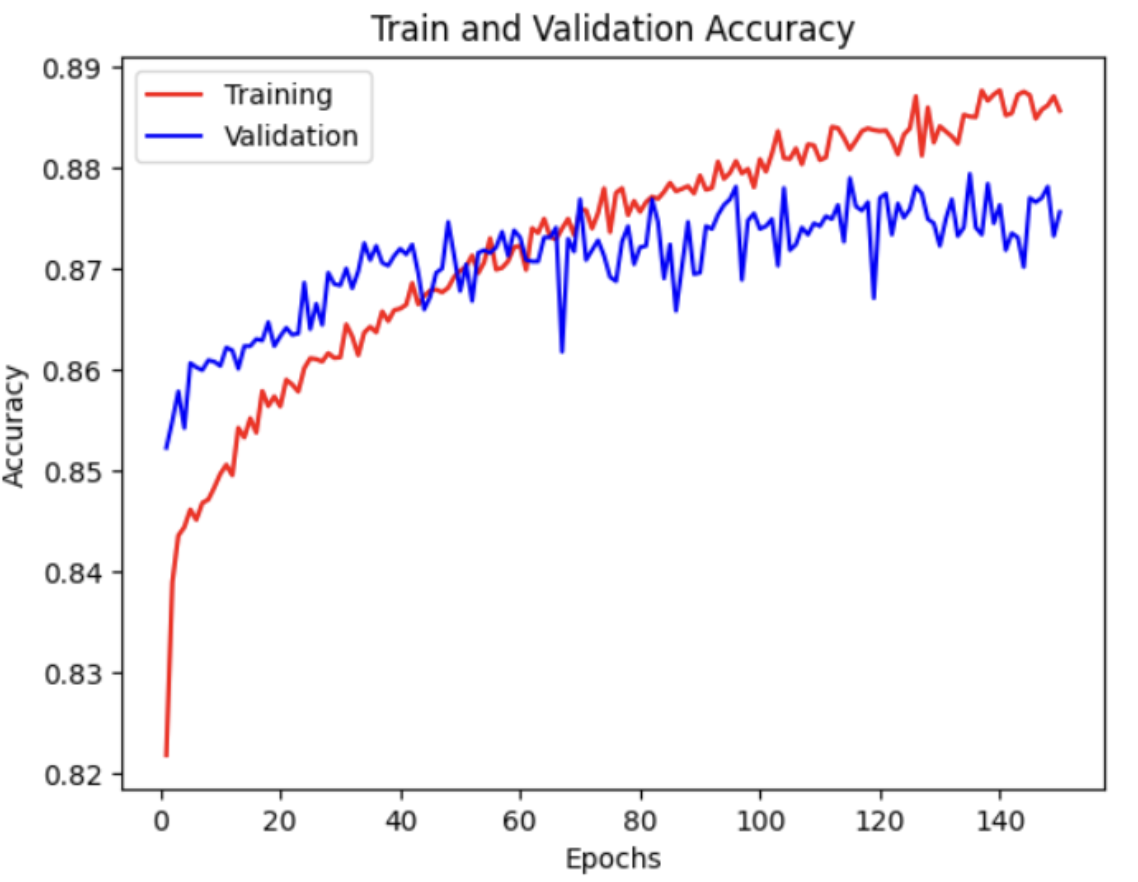
\includegraphics[width=0.45\textwidth]{images/robertaAccuracyFigureY150Epoch.png}
    \caption{Training and validation accuracy of the RoBERTa-Twitter model during classification head training}
    \label{fig:roberta_accuracy_finetune}
\end{figure}



Regarding the loss, it can be observed that around epoch 70, overfitting begins, as the validation loss stops decreasing or even starts to increase, while the training loss continues to drop rapidly. 

Concerning accuracy, it is noticeable that around epoch 70, the validation accuracy plateaus, whereas the training accuracy continues to improve. 

In summary, on the validation set, the loss stabilizes around 0.3 and the accuracy around 0.875, exhibiting an oscillatory behavior. The best validation accuracy was reached at epoch 135, with a value of 0.87937.

\begin{table}[H]
\centering
\caption{Classification Report after Training the Classification Head}
\label{tab:classification_report_2}
\begin{tabular}{lcccc}
\toprule
Class        & Precision & Recall & F1-score & Support \\
\midrule
0.0          & 0.85      & 0.91   & 0.88     & 3462    \\
1.0          & 0.91      & 0.84   & 0.88     & 3693    \\
\midrule
Accuracy     &           &        & 0.88     & 7155    \\
Macro Avg    & 0.88      & 0.88   & 0.88     & 7155    \\
Weighted Avg & 0.88      & 0.88   & 0.88     & 7155    \\
\bottomrule
\end{tabular}
\end{table}

\begin{figure}[H]
    \centering
    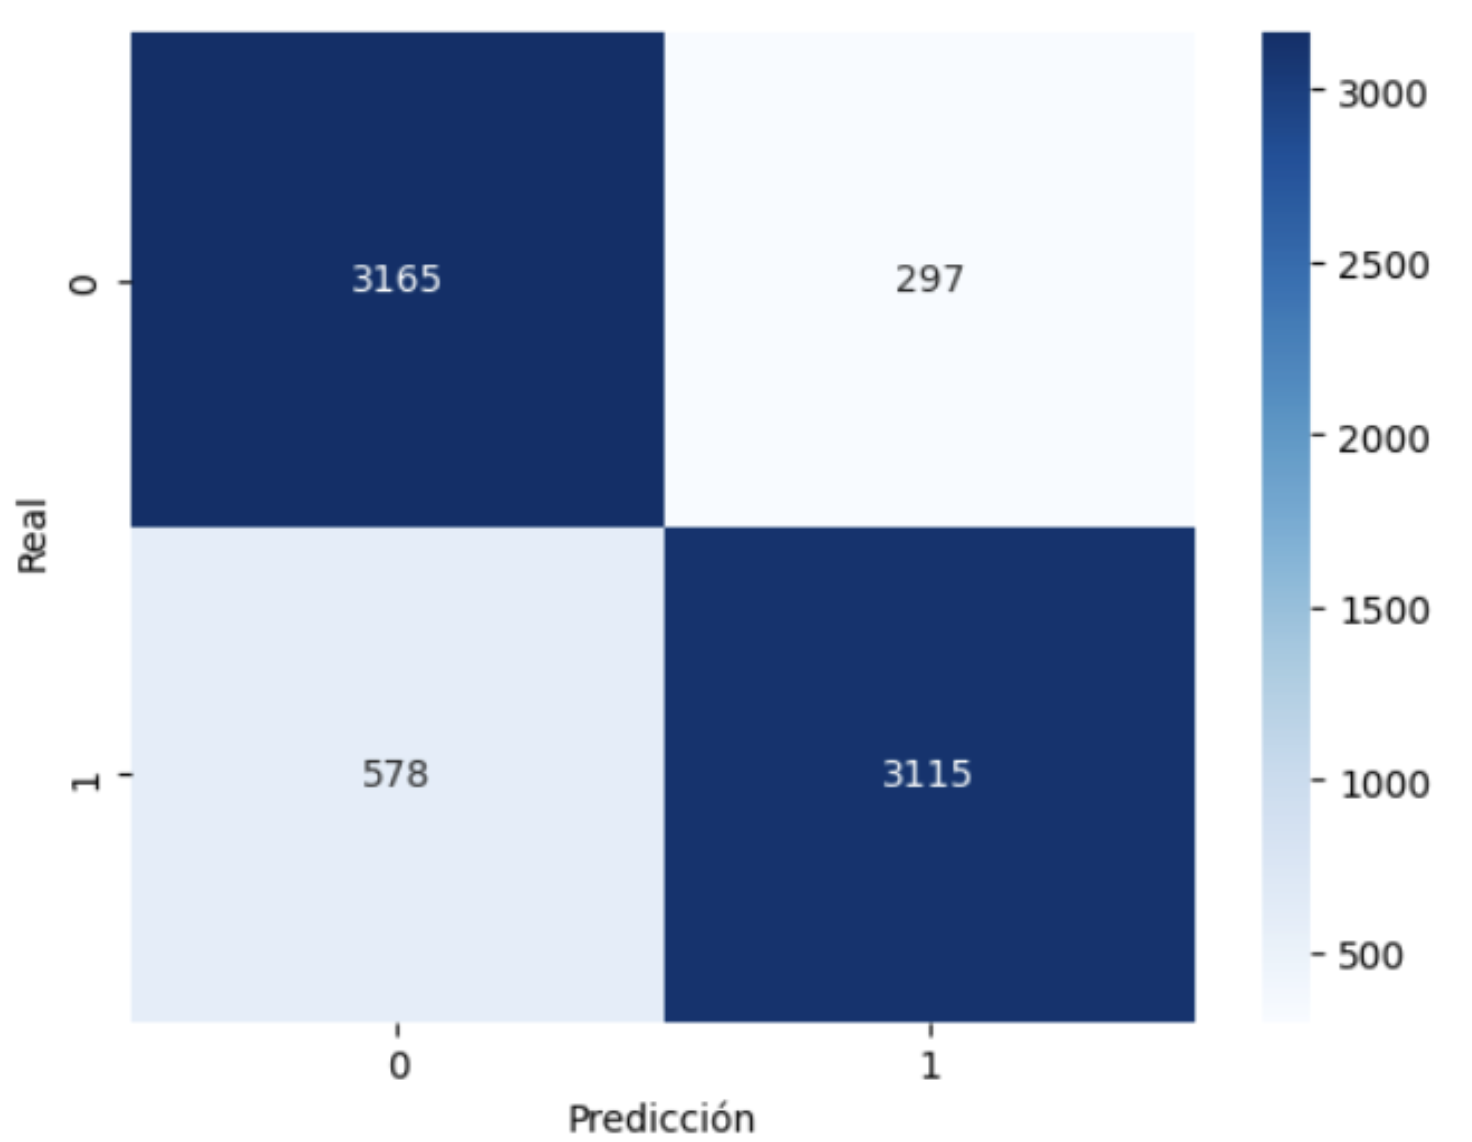
\includegraphics[width=0.45\textwidth]{images/robertaConfusionMatrix.png} 
    \caption{Confusion matrix of the RoBERTa-Twitter model}
    \label{fig:roberta_confusion_matrix}
\end{figure}

In previos charts, the classification report from the first training stage is shown. This report once again reflects a pattern observed in other models: low precision for the negative class, which results in low recall for the positive class. 

However, a surprising accuracy of 88\% was achieved by training only the designed classification head. This is supported by the confusion matrix in Figure X, where a high concentration of correct predictions and a reduced number of errors can be observed.

Based on the results from the first training phase, the model with the best validation accuracy was selected for the second stage. In this phase, all weights were unfrozen, and training continued for 100 epochs, saving the best-performing model.


\begin{figure}[H]
    \centering
    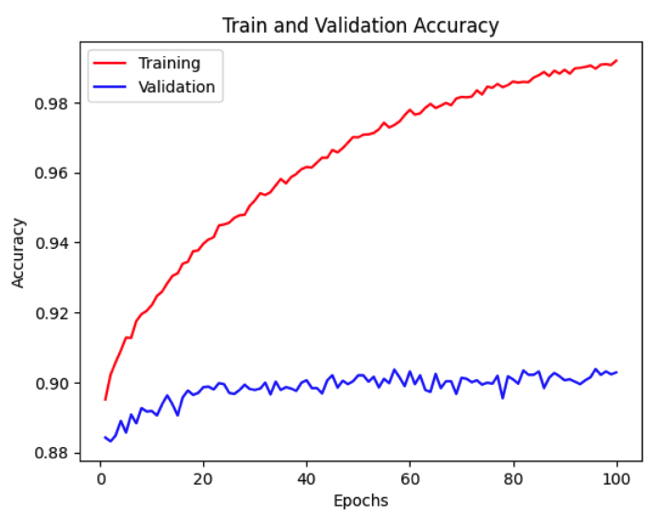
\includegraphics[width=0.45\textwidth]{images/robertaValidationAccuray100Epoch.png}
    \caption{Validation accuracy of the RoBERTa-Twitter model during full fine-tuning (100 epochs)}
    \label{fig:roberta_validation_accuracy_100epoch}
\end{figure}

\begin{figure}[H]
    \centering
    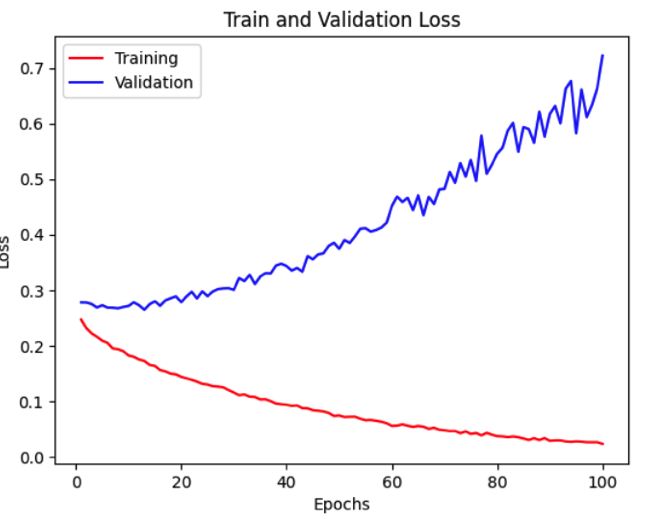
\includegraphics[width=0.45\textwidth]{images/robertaValidationLost100Epoch.png}
    \caption{Validation loss of the RoBERTa-Twitter model during full fine-tuning (100 epochs)}
    \label{fig:roberta_validation_loss_100epoch}
\end{figure}

Figures \ref{fig:roberta_validation_accuracy_100epoch} and \ref{fig:roberta_validation_loss_100epoch} show the evolution of loss and accuracy over the 100 training epochs. Overfitting can be observed in both loss and accuracy: the model continues to improve on the training set while deteriorating on the validation set. 

The validation loss increases rapidly, while the validation accuracy decreases more gradually. Nevertheless, the performance on the validation set improved, reaching a validation accuracy of 0.90383 at epoch 96.

\begin{table}[H]
\centering
\caption{Classification Report after Full Fine-Tuning}
\label{tab:classification_report_final}
\begin{tabular}{lcccc}
\toprule
Class        & Precision & Recall & F1-score & Support \\
\midrule
0.0          & 0.88      & 0.93   & 0.90     & 3462    \\
1.0          & 0.93      & 0.88   & 0.91     & 3693    \\
\midrule
Accuracy     &           &        & 0.90     & 7155    \\
Macro Avg    & 0.91      & 0.91   & 0.90     & 7155    \\
Weighted Avg & 0.91      & 0.90   & 0.90     & 7155    \\
\bottomrule
\end{tabular}
\end{table}


\begin{figure}[H]
    \centering
    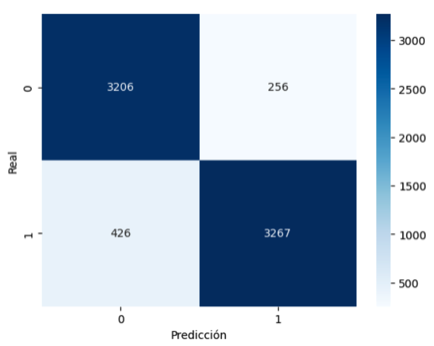
\includegraphics[width=0.45\textwidth]{images/robertaConfusionMatrix100Epochs.png} 
    \caption{Confusion matrix of the RoBERTa-Twitter model after full fine-tuning (100 epochs)}
    \label{fig:roberta_confusion_matrix_100epochs}
\end{figure}

As shown in Table \ref{tab:classification_report_final} and Figure \ref{fig:roberta_confusion_matrix_100epochs}, both the classification report and the confusion matrix are presented. These results reveal the issue of bias toward the negative class, a pattern seen in previous models. 

Nevertheless, the model achieves a remarkable performance of 90\% accuracy, which could be considered a potential solution to the problem. However, this result, while close, does not surpass the 92.38\% reported in \cite{fieri2023offensive}.


\subsection{Naive Bayes Results}

\begin{table}[H]
\centering
\caption{Classification Report for Naïve Bayes Classifier using TF-IDF features}
\label{tab:nb_classification_report}
\begin{tabular}{lcccc}
\toprule
Class        & Precision & Recall & F1-score & Support \\
\midrule
0            & 0.85      & 0.83   & 0.84     & 4654    \\
1            & 0.84      & 0.86   & 0.85     & 4887    \\
\midrule
Accuracy     &           &        & 0.85     & 9541    \\
Macro Avg    & 0.85      & 0.85   & 0.85     & 9541    \\
Weighted Avg & 0.85      & 0.85   & 0.85     & 9541    \\
\bottomrule
\end{tabular}
\end{table}

\begin{figure}[H]
    \centering
    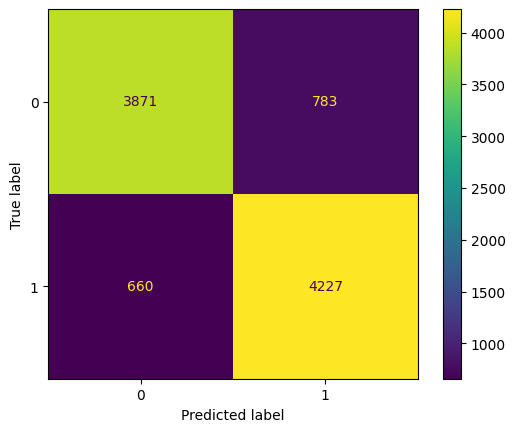
\includegraphics[width=0.45\textwidth]{images/confusion_matrix_nb.png}
    \caption{Confusion matrix for the Naïve Bayes model using TF-IDF features}
    \label{fig:confusion_nb}
\end{figure}

\begin{figure}[H]
    \centering
    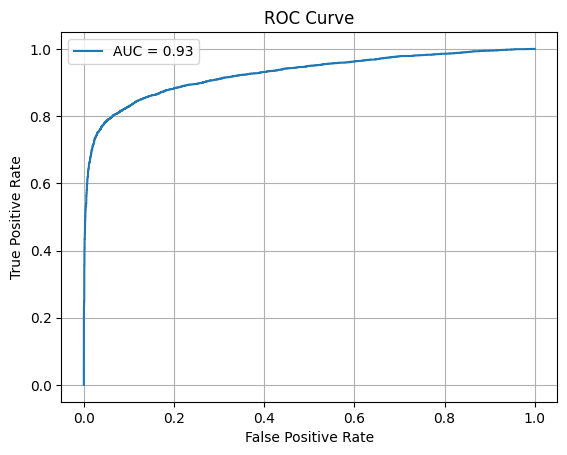
\includegraphics[width=0.45\textwidth]{images/roc_curve_nb.png}
    \caption{ROC curve for the Naïve Bayes classifier with an AUC of 0.93}
    \label{fig:roc_nb}
\end{figure}


The Naïve Bayes classifier achieved competitive results using TF-IDF representations as input features. As shown in Table~\ref{tab:nb_classification_report}, the model attained a balanced performance across both classes, with an F1-score of 0.84 for class 0 (non-hate) and 0.85 for class 1 (hate). The overall accuracy was 85\%, which is comparable to more complex architectures, demonstrating the effectiveness of probabilistic models for text classification tasks with well-engineered features.

The confusion matrix in Figure~\ref{fig:confusion_nb} shows that the classifier correctly predicted 3871 non-hate and 4227 hate speech instances. However, it also misclassified 660 hate comments as non-hate and 783 non-hate comments as hate, indicating a slightly better recall for the hate class.

Furthermore, the ROC curve in Figure~\ref{fig:roc_nb} presents an Area Under the Curve (AUC) of 0.93, which confirms the model’s strong ability to discriminate between classes across different thresholds. This result highlights the classifier’s reliability in ranking predictions, making it a viable choice for lightweight and interpretable hate speech detection systems.

Despite its simplicity and the conditional independence assumption, the Naïve Bayes classifier provides robust performance, especially when computational efficiency is prioritized or in ensemble learning contexts.


\subsection{GRU Results}

\begin{table}[H]
\centering
\caption{Classification Report for GRU model using CLS token embeddings}
\label{tab:gru_classification_report}
\begin{tabular}{lcccc}
\toprule
Class        & Precision & Recall & F1-score & Support \\
\midrule
0            & 0.87      & 0.93   & 0.90     & 4953    \\
1            & 0.92      & 0.87   & 0.89     & 5084    \\
\midrule
Accuracy     &           &        & 0.90     & 10037   \\
Macro Avg    & 0.90      & 0.90   & 0.90     & 10037   \\
Weighted Avg & 0.90      & 0.90   & 0.90     & 10037   \\
\bottomrule
\end{tabular}
\end{table}

\begin{figure}[H]
    \centering
    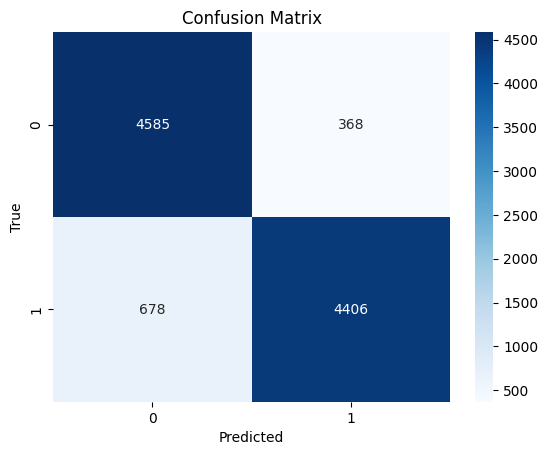
\includegraphics[width=0.45\textwidth]{images/confusion_matrix_gru.png}
    \caption{Confusion matrix for GRU model using CLS embeddings}
    \label{fig:confusion_gru}
\end{figure}

\begin{figure}[H]
    \centering
    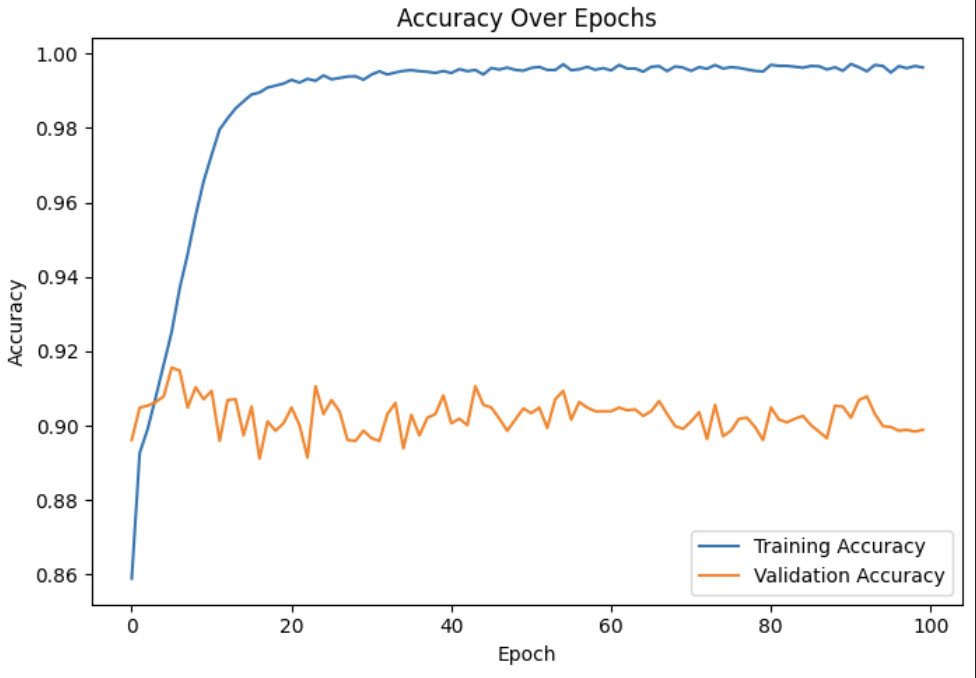
\includegraphics[width=0.45\textwidth]{images/accuracy_over_epoch_gru.png}
    \caption{Accuracy over epochs for the GRU model.}
    \label{fig:accuracy_gru}
\end{figure}

\begin{figure}[H]
    \centering
    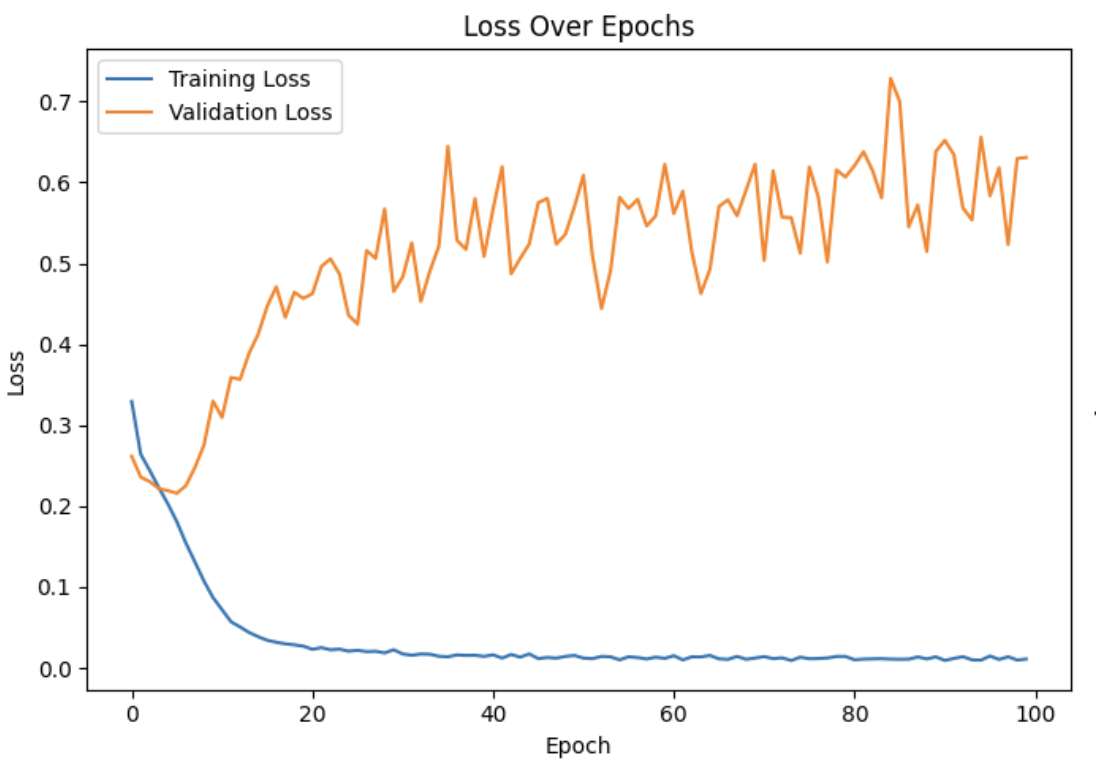
\includegraphics[width=0.45\textwidth]{images/lossOverEpochGRU.png}
    \caption{Loss over epochs for the GRU model.}
    \label{fig:loss_gru}
\end{figure}


\begin{figure}[H]
    \centering
    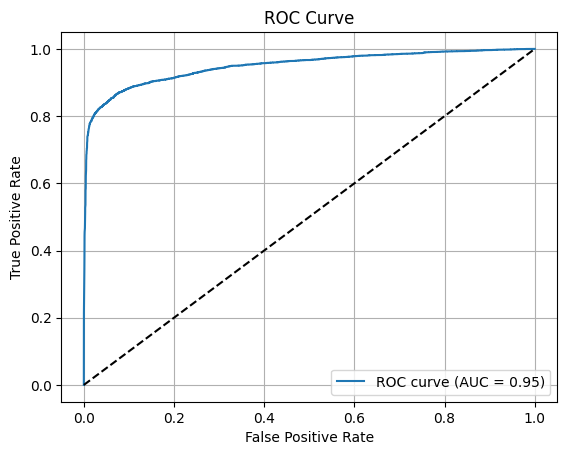
\includegraphics[width=0.45\textwidth]{images/roc_curve_gru.png}
    \caption{ROC curve for GRU model}
    \label{fig:roc_gru}
\end{figure}

\begin{figure}[H]
    \centering
    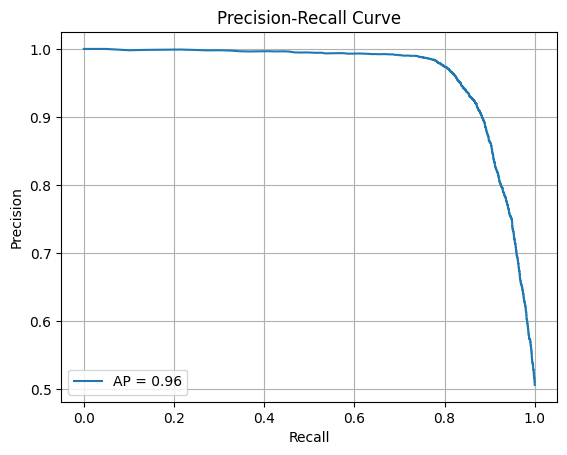
\includegraphics[width=0.45\textwidth]{images/precision_recall_gru.png}
    \caption{Precision-Recall curve for GRU model with AP = 0.96}
    \label{fig:pr_gru}
\end{figure}

The GRU model trained on CLS token embeddings demonstrated strong classification performance, achieving an overall accuracy of 90\% and an F1-score of 0.89 for the hate speech class (Table~\ref{tab:gru_classification_report}). The model showed balanced performance across both classes, with precision and recall values above 0.87. The confusion matrix in Figure~\ref{fig:confusion_gru} illustrates this balance, with 4585 true negatives and 4406 true positives, though 678 hate examples were misclassified as non-hate.

Despite the strong predictive performance, the training curves in Figure~\ref{fig:training_curves_gru} indicate potential overfitting. The training loss decreases consistently, but the validation loss remains high and fluctuates significantly across epochs. Similarly, the training accuracy approaches 99\% while validation accuracy stabilizes near 90\%, suggesting that the model has learned the training data very well but may not generalize perfectly to unseen data.

Nevertheless, the ROC curve in Figure~\ref{fig:roc_gru} shows excellent separability between classes, with an AUC close to 0.93. The Precision-Recall curve in Figure~\ref{fig:pr_gru} further supports this, with an average precision (AP) of 0.96, indicating that the model maintains high precision across a wide range of recall thresholds. These metrics confirm that the GRU model is effective at ranking and identifying hate speech with high confidence, even under class imbalance conditions.

\section{Conclusions}
Taking into account all the previously mentioned results and their comparison with related works, we can say that some of our models outperformed certain previous investigations in terms of accuracy. However, there were also investigations where our metrics fell short. Our best accuracy was achieved using the model based on RoBERTa through fine-tuning, as shown in Table X. With this model, we were able to reach 90\% accuracy, which is a high score, but still considerably lower compared to results like those obtained by \citep{fieri2023offensive}, where 96.102\% was achieved using BI-LSTM and EDA.

Our 90\% accuracy can be problematic in terms of misclassification. If it occurs, we might end up suppressing freedom of speech or failing to identify inappropriate, hateful, or toxic content. The most significant concern with the resulting model is the possibility of marking something as non-toxic when it is actually toxic, considering the precision and recall values obtained.

Another insight derived from our results is that deep learning seems to be better suited for this kind of NLP task. As shown in Table X, the best results and improvements were obtained using DL-based architectures. This leads us to think that the ability to sequentially analyze a sentence and/or transform it through different optimized feature spaces contributes to better characteristic and insight extraction, which in turn results in better performance on the task. Additionally, given that our best-performing model was a fine-tuned version of RoBERTa, we can say that the robustness of DL architectures considerably boosts the results, especially when pre-training (transfer learning) is involved.

To improve our results, multiple approaches can be explored in future investigations. One of these could be training on more data, particularly data from the toxic class, as our models appear to be biased toward the non-toxic class. Another possibility could involve testing and fine-tuning decoders for the classification task through conditional generation based on a given sentence or context.

\bibliographystyle{plainnat}
\bibliography{references}

\end{document}